\section{Développement de l'application}
Ce point du rapport est dédié au déroulement du développement de l'application \textit{Manabu}. J'expliquerai ce que j'ai mis en place point par point, en fonction des différentes parties de l'application. Je commencerai par énoncer quelques généralités concernant le programme, puis j'expliquerai le menu principal, et enfin les différents exercices au niveau facile, le 1. J'illustrerai au maximum mes propos par des screenshots\footnote{Ceux-ci ont été pris sur la Nvidia Shield Tablet, qui a une résolution de 1920*1200 pixels.} des différents exercices.

\subsection{Généralités}
Par généralités, il faut entendre les décisions que j'ai prises et qui affectent l'application dans son ensemble ou simplement des points nécessitant d'être explicités pour une meilleure compréhension du développement de l'application.\\

Tout d'abord, avant de me lancer dans la création de \textit{Manabu}, j'ai suivi le premier tutoriel disponible sur le site officiel d'Android pour les développeurs, \textit{Building Your First App}\footnote{Building Your First App, \url{http://developer.android.com/training/basics/firstapp/index.html}, consulté en janvier et février 2015}. Ceci m'a permis de me familiariser avec le SDK Android et de connaître les bases de ce type de programmation.\\

Ensuite, il faut savoir que \textit{Manabu} est composée de 5 activités. Une activité, comme expliqué au point \textit{Outils et technologies utilisés} dans la définition d'Android Developer, représente un écran avec lequel l'utilisateur peut interagir. Dans la pratique, une activité est contenue dans une classe java qui lui est propre et associée avec un où plusieurs layouts. Dans le cas présent, j'ai considéré que mon application est constituée de 5 parties différentes. J'ai donc transcrit chacune d'entre elles en une activité. Celles-ci sont :
\begin{itemize}
\item la \textit{main activity}, autrement dit le menu principal. Il s'agit de l'écran d'ouverture de l'application;
\item l'activité de l'exercice \textit{Imagerie};
\item l'activité de l'exercice \textit{Lecture flash};
\item l'activité de l'exercice \textit{Anagrammes};
\item l'activité de l'exercice \textit{Écouter le son}.
\end{itemize}
Toute ces activités sont définies en plein écran et en orientation paysage par défaut. Il est impossible de jouer à \textit{Manabu} en mode portrait. J'ai forcé le cette orientation car il est possible d'y aligner plus d'éléments les uns à la suite des autres. C'est plus efficace quand les mots sont longs.\\

L'activité contenant le menu principal ne contient qu'un seul layout. Les autres activités, celles des exercices, en contiennent quant à elles plusieurs. Trois layouts sont communs au quatre exercices. Il s'agit du layout du menu de démarrage (Fig. \ref{dem}), du layout d'affichage des règles du jeu (Fig. \ref{regles}) et du layout de fin d'exercice (Fig. \ref{fin}). Le layout de démarrage contient des boutons permettant de choisir le niveau, un bouton pour afficher les règles du jeu, et un bouton pour démarrer l'exercice. Le layout des règles contient en haut à droite un bouton permettant d'écouter les règles du jeu, au centre le texte des règles, et en bas un bouton pour revenir au layout des règles et un bouton pour démarrer le jeu. Le layout de fin d'exercice contient quant à lui un texte de félicitation du joueur, ainsi que deux boutons proposant le choix de soit revenir au menu principal, soit rejouer à l'exercice.\\

En outre, concernant les règles du jeu, j'ai rendu leur consultation également possible depuis les exercices déjà démarrés. Pour ce faire, j'ai placé en haut à gauche des layouts propres aux différents exercices un bouton "?". Un clic sur celui-ci ouvre un pop-up (Fig. \ref{popup}) ré-expliquant les règles du jeu.\\

\begin{figure}[H]
\centering
\begin{subfigure}[t]{8.5cm}
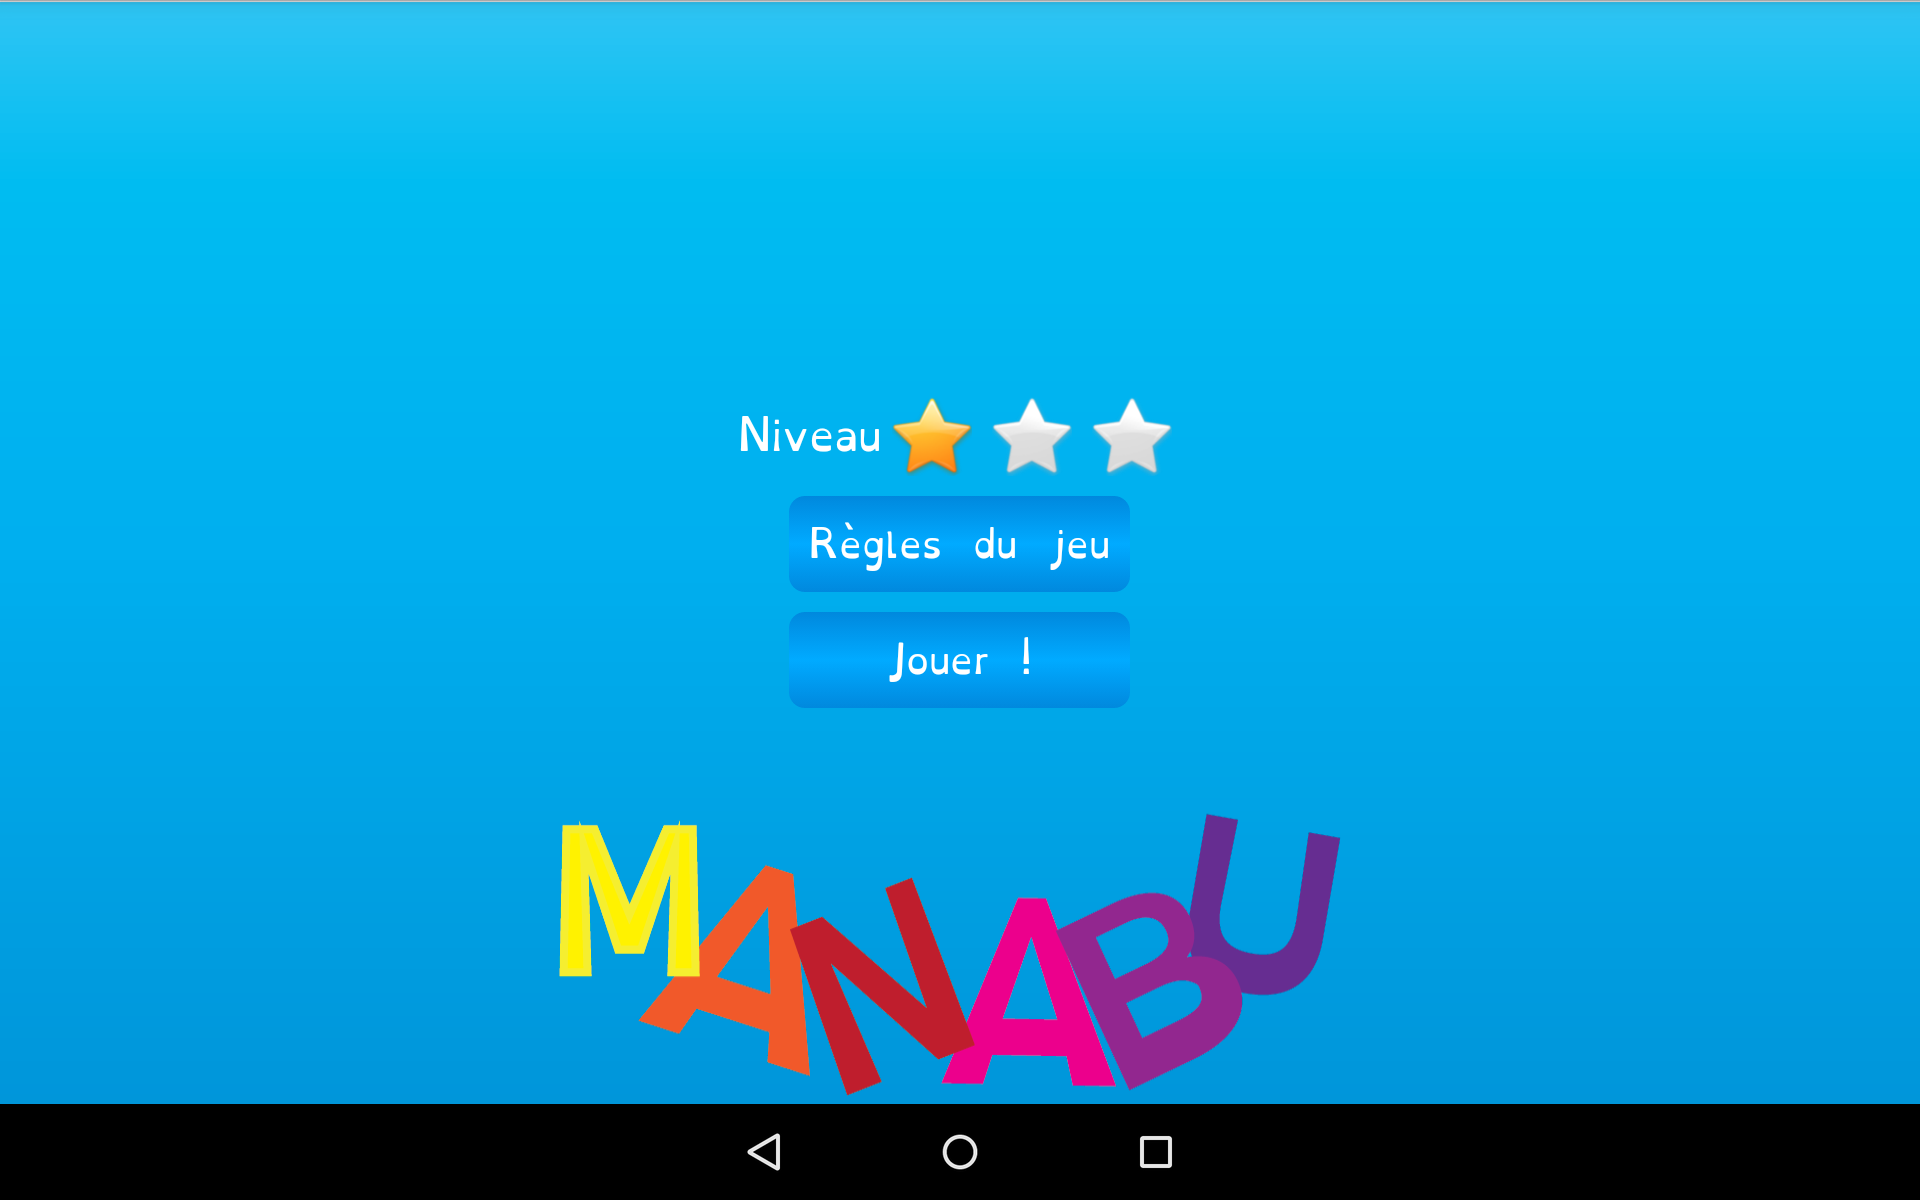
\includegraphics[width=8.5cm]{img/layout-debut.png}
\caption{Layout du menu de démarrage}
\label{dem}
\end{subfigure}
~
\begin{subfigure}[t]{8.5cm}
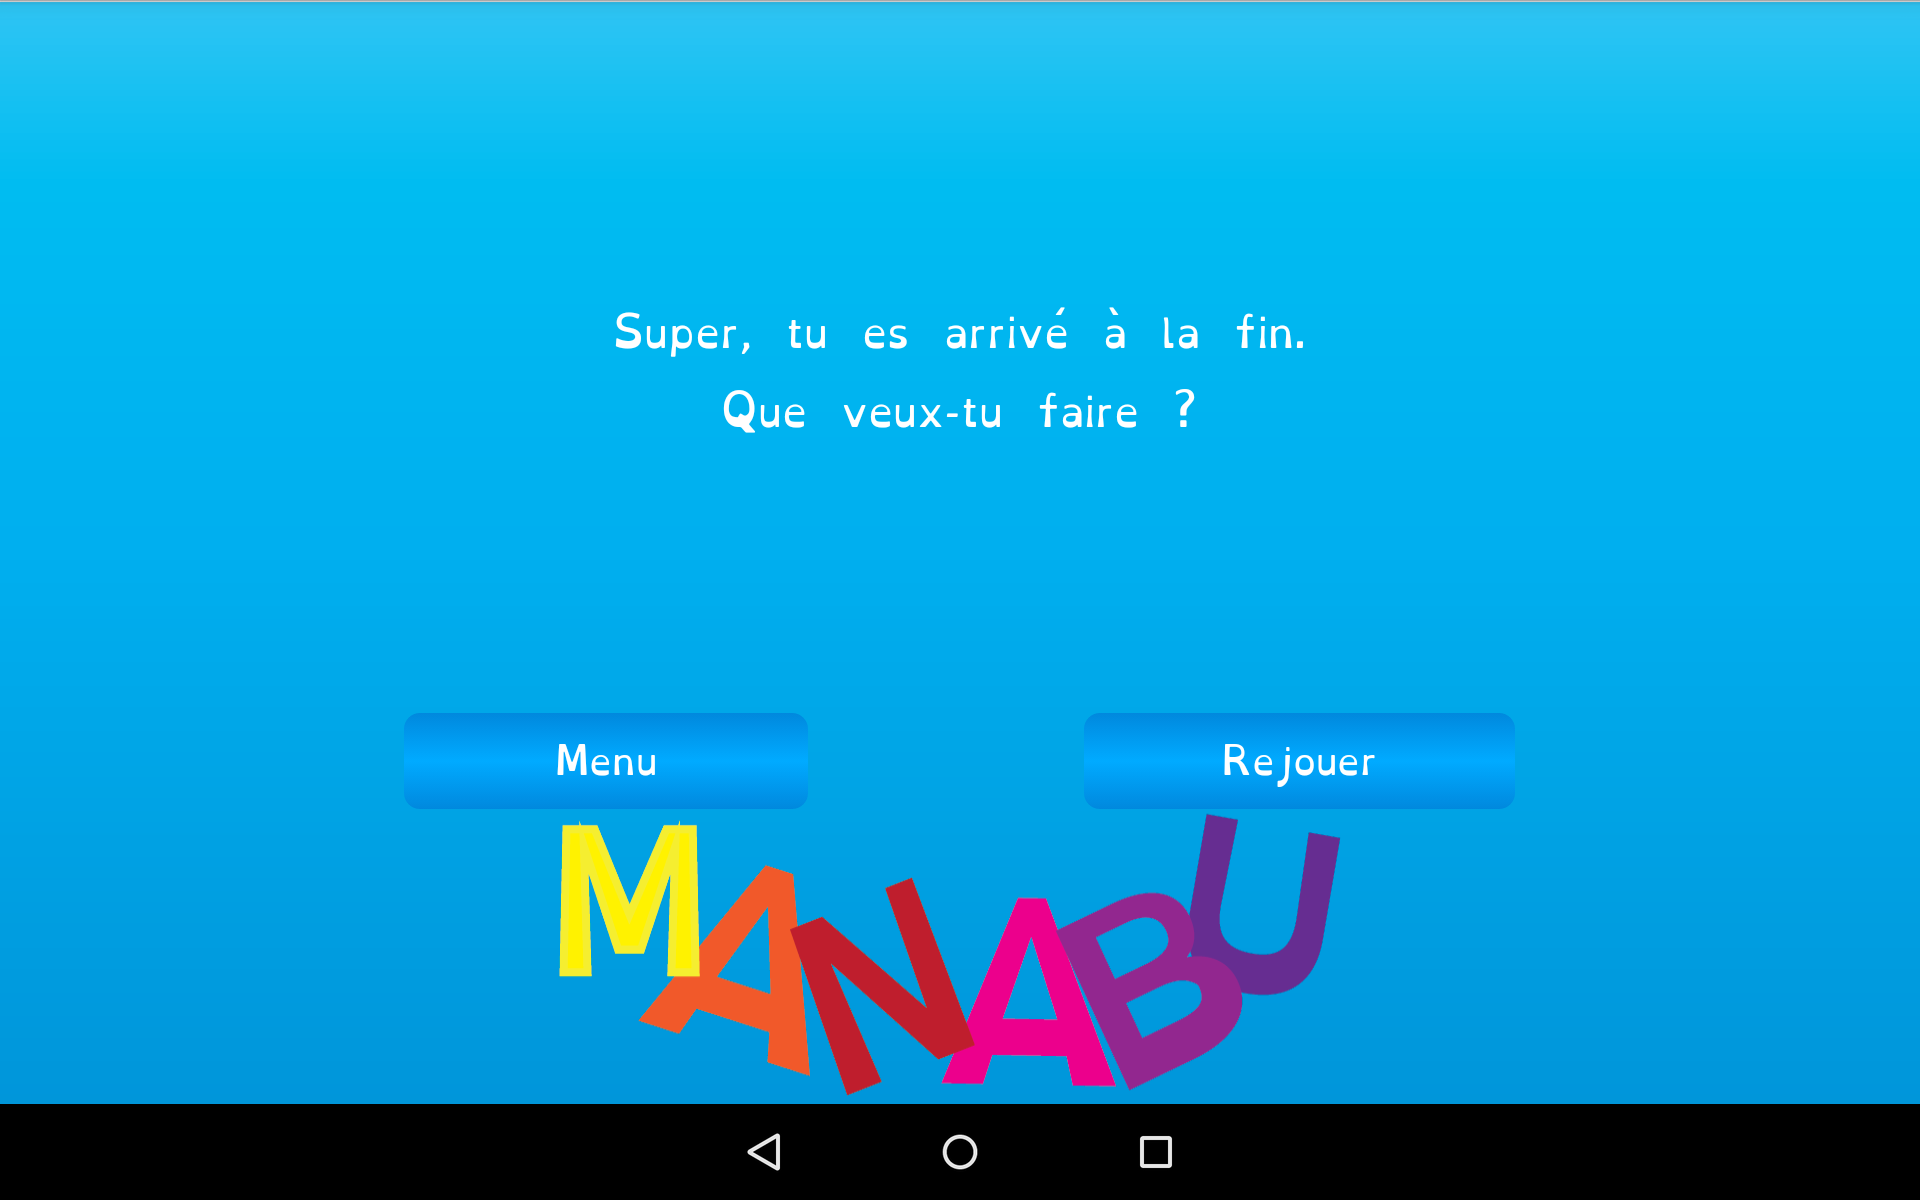
\includegraphics[width=8.5cm]{img/layout-fin.png}
\caption{Layout de fin d'exercice}
\label{fin}
\end{subfigure}
~
\begin{subfigure}[t]{8.5cm}
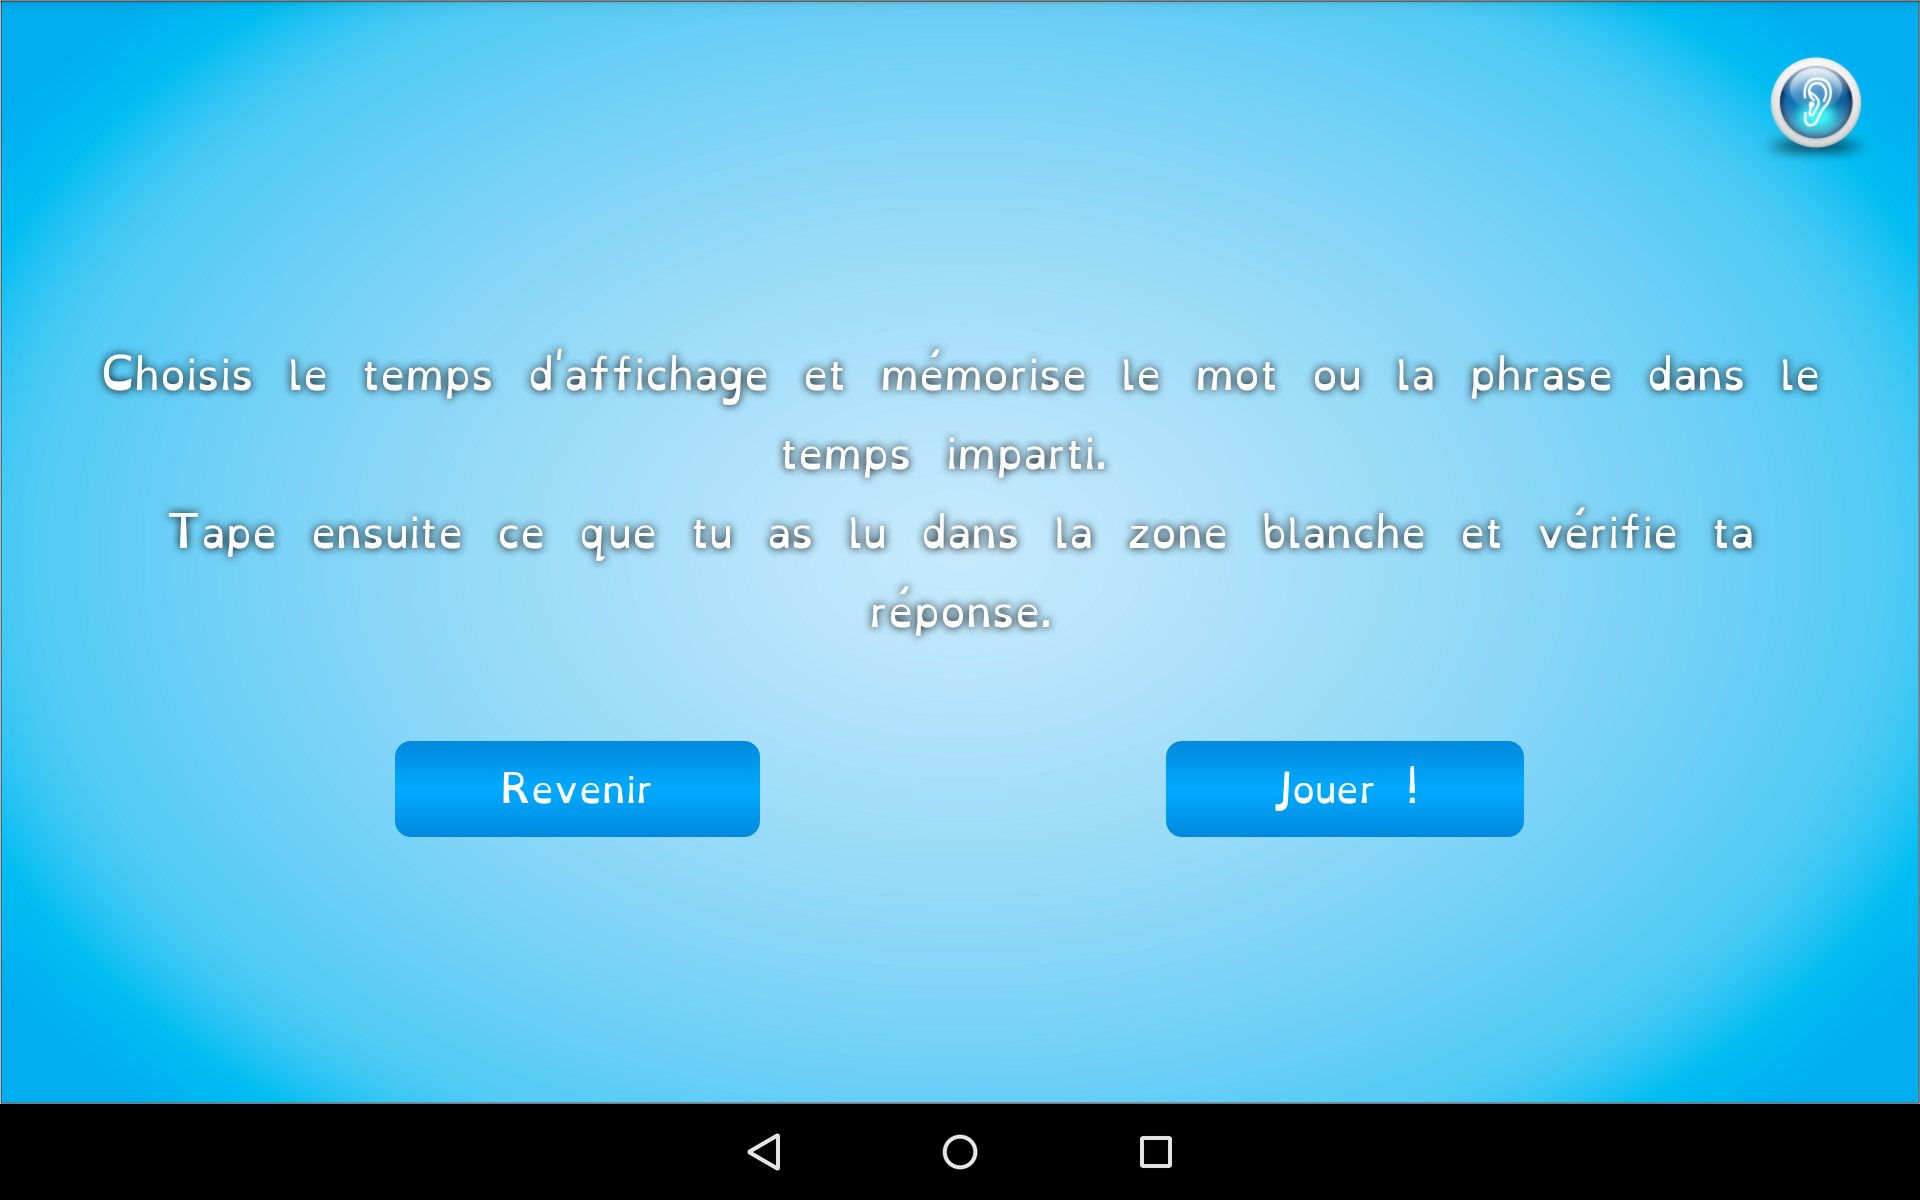
\includegraphics[width=8.5cm]{img/layout-regles.png}
\caption{Layout d'affichage des règles}
\label{regles}
\end{subfigure}
~
\begin{subfigure}[t]{8.5cm}
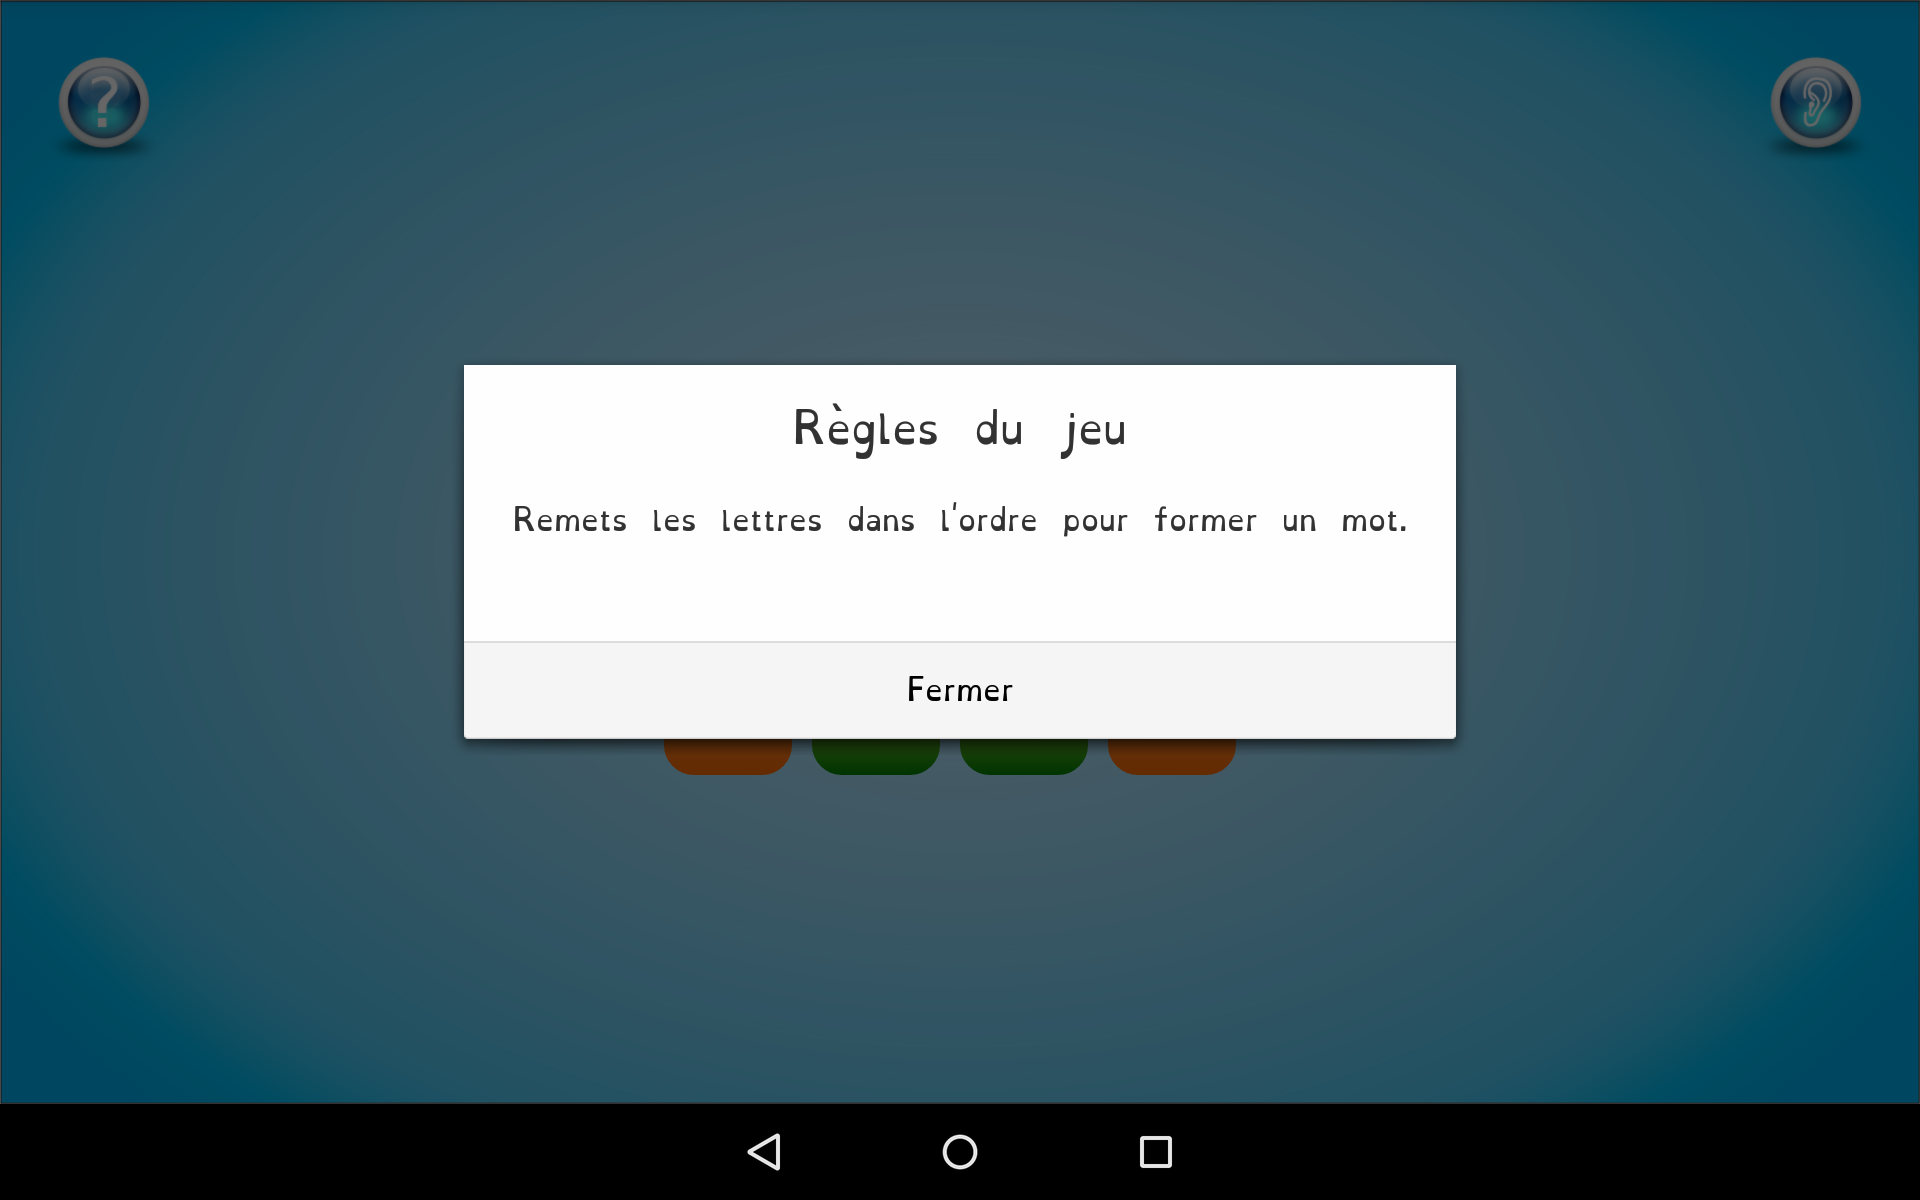
\includegraphics[width=8.5cm]{img/popup.png}
\caption{Pop-up d'affichage des règles}
\label{popup}
\end{subfigure}
\caption{Différents layouts communs et pop-up avec les règles}
\end{figure}

Par ailleurs, j'ai intégré \textit{OpenDyslexic} en tant que police principale de \textit{Manabu}. Ça n'a pas été la tâche la plus simple. J'ai tout d'abord essayé de modifier la police d'un élément (pensant par la suite pouvoir l'appliquer à toute l'application) via la méthode "classique". C'est-à-dire aller chercher la police dans un dossier et l'appliquer à chaque élément voulu. Cette méthode s'est révélée lourde à mettre en place. C'est en voulant intégrer par la suite la librairie \textit{Calligraphy} de ChrisJenx\footnote{Disponible gratuitement sur GitHub à l'adresse \url{https://github.com/chrisjenx/Calligraphy}.} permettant d'utiliser une police pour toute l'application facilement que j'ai rencontré le problème avec Maven dans Eclipse. J'ai donc, comme dit précédemment, changé d'IDE pour Android Studio. Gradle a quant à lui ajouté sans problème la librairie à la liste des dépendances.\\

En dernier lieu, j'ai choisi d'exécuter plusieurs fois le même exercice lors du démarrage de celui-ci. Je trouve que devoir à chaque fois ré-appuyer sur le bouton pour recommencer est dérangeant. De ce fait, je lance les exercices par série de 10. Lorsque le premier est réussi, il passe automatiquement au suivant, et ainsi de suite.\\

Enfin, je ne présenterai ici que le premier niveau implémenté pour chaque exercice. L'algorithme des niveaux supérieurs étant identique (ou quasi) à celui du niveau facile, je ne juge pas nécessaire d'expliquer leurs mises en place.

\subsection{Le menu principal}
Le menu principal représente l'activité de base de l'application, celle depuis laquelle peuvent être démarrées les autres activités contenant les exercices. Le layout formant ce menu est relativement simple (Fig. \ref{menu}). Il s'agit de quatre boutons disposés en un rectangle. Chacun des boutons lance un des exercices.\\

Pour chaque bouton, il m'a fallu implémenter une fonction spécialisée permettant de lancer la nouvelle activité correspondant à l'exercice désiré.
Lancer une nouvelle activité se fait à l'aide d'un \textit{intent}. Un intent est une sorte de lien de communication pour le système Android. Celui-ci signale qu'il se passe quelque chose. Dans le cas présent, l'intent signale que l'activité du menu principal va en démarrer une autre.\\

Enfin, je tiens à mentionner qu'il n'est pas possible de lancer les activités de plusieurs exercices à la fois. En effet, lorsqu'un exercice est lancé depuis le menu, l'activité en cours représentée passe du menu à l'activité de l'exercice, l'activité menu étant alors en attente. Il faut quitter l'exercice, et donc l'activité, pour revenir au menu et pouvoir en démarrer une autre.

\begin{figure}[H]
\centering
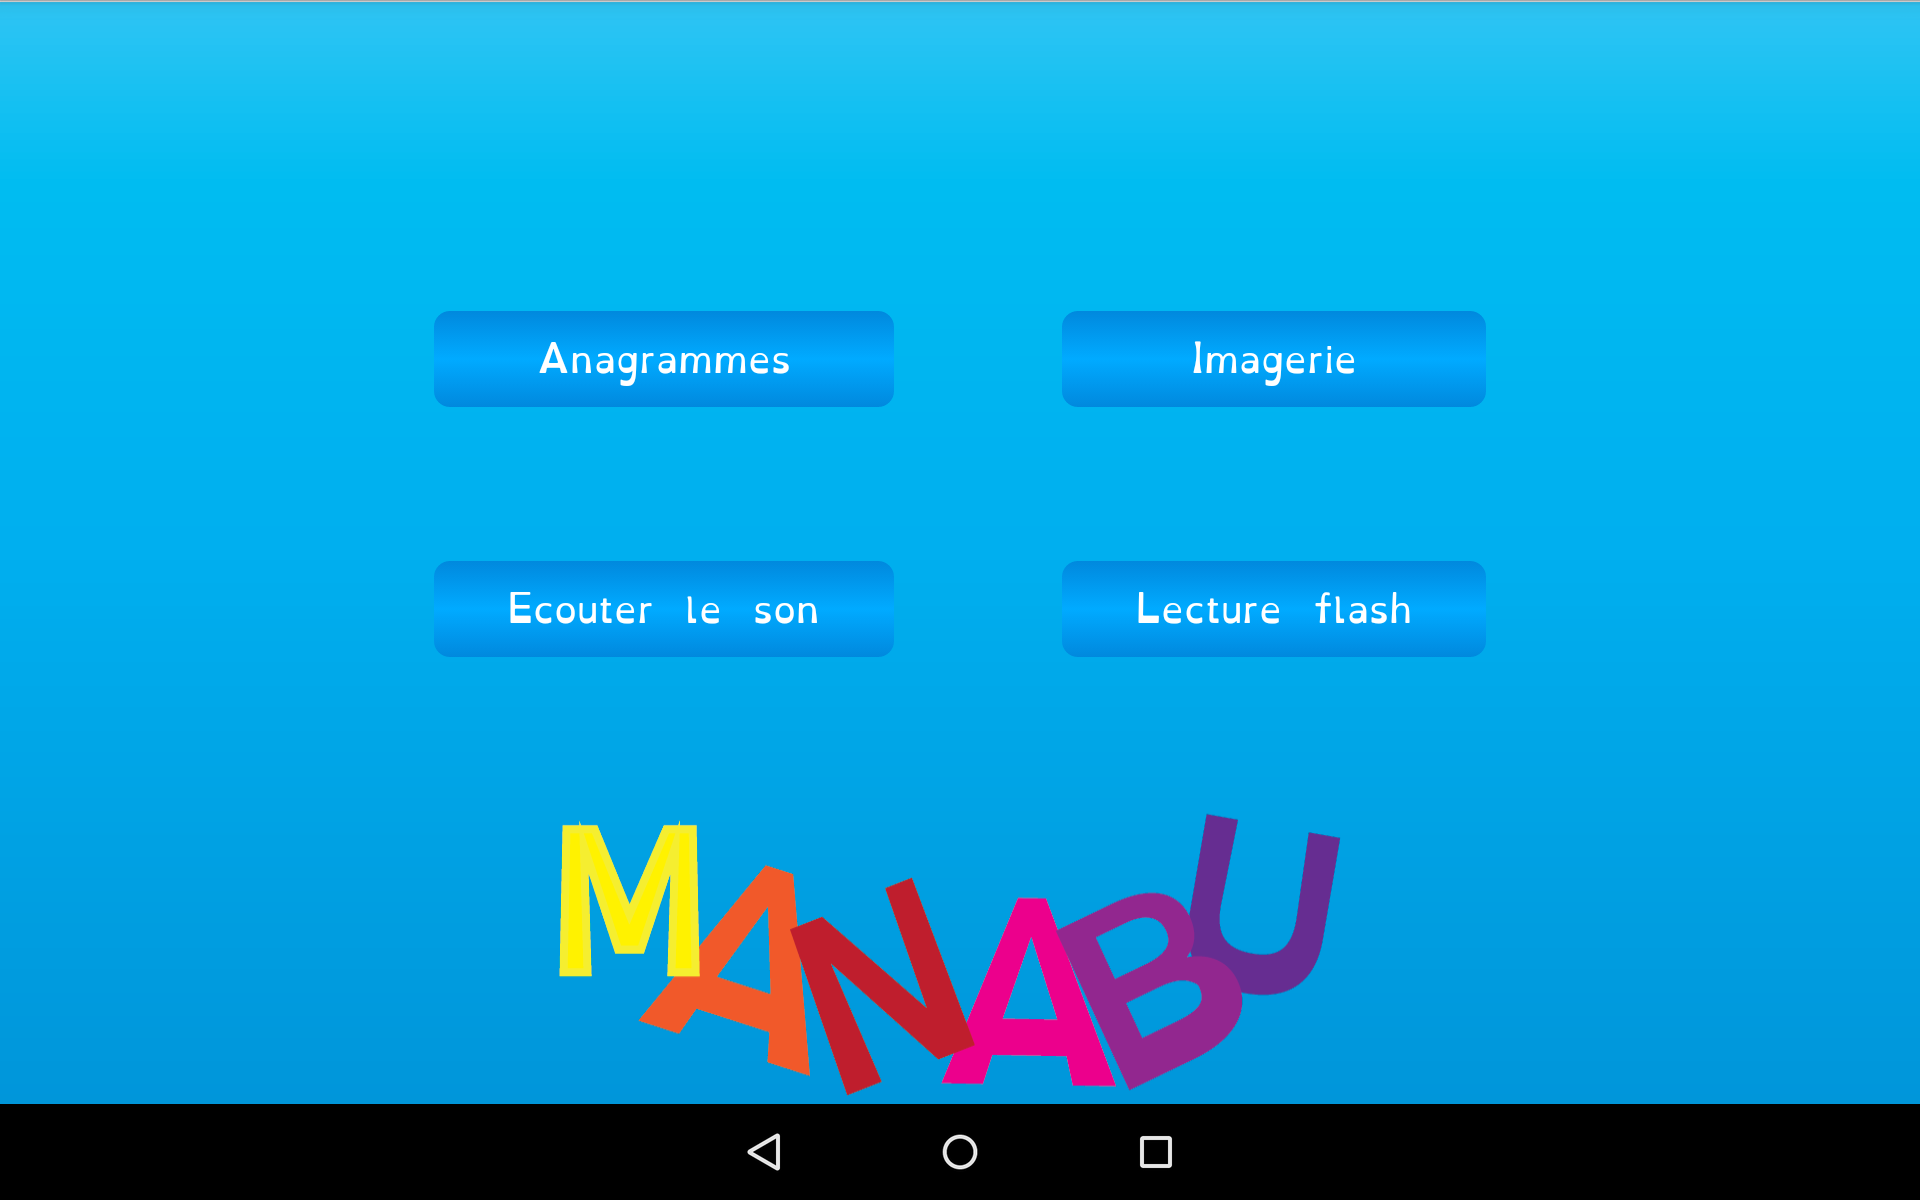
\includegraphics[width=10cm]{img/menu.png}
\caption{Menu principal}
\label{menu}
\end{figure}

\subsection{L'exercice \textit{Imagerie}}
L'exercice \textit{Imagerie} est le premier que j'ai choisi d'implémenter. Il s'agit de mon exercice favori, car il m'a permis d'exprimer ma créativité au travers des dessins réalisés. Pour le premier niveau, j'ai choisi de me baser sur la version la plus simple des fichiers Freinet : une image affichée avec un mot à mémoriser, et puis, sur base de la même image, retrouver ce mot parmi trois propositions.\\

Afin de réaliser ce niveau 1, il m'a fallu définir la liste de mots qui allaient être utilisés. J'ai déterminé une liste d'une vingtaine de mots à illustrer. Pour chacun de ceux-ci, j'ai également choisi deux autres mots ressemblant à la bonne réponse pour faire office de fausses réponses. J'ai réalisé les illustrations dans un style de dessin simple, à l'aide du logiciel de dessin vectoriel Adobe Illustrator. \\


En ce qui concerne la partie programmation de l'exercice, celui-ci contient deux layouts XML qui lui sont spécifiques. Le premier layout présente l'affichage de l'image et du mot à retenir, ainsi qu'un bouton "\textit{Mémorisé}" (Fig. \ref{imgS}). Ce bouton permet de passer au layout suivant. Ce dernier est constitué de la même image que pour le premier layout, ainsi que trois boutons représentant le choix des mots (Fig. \ref{imgF}).\\

\begin{figure}[H]
\centering
\begin{subfigure}[t]{8.5cm}
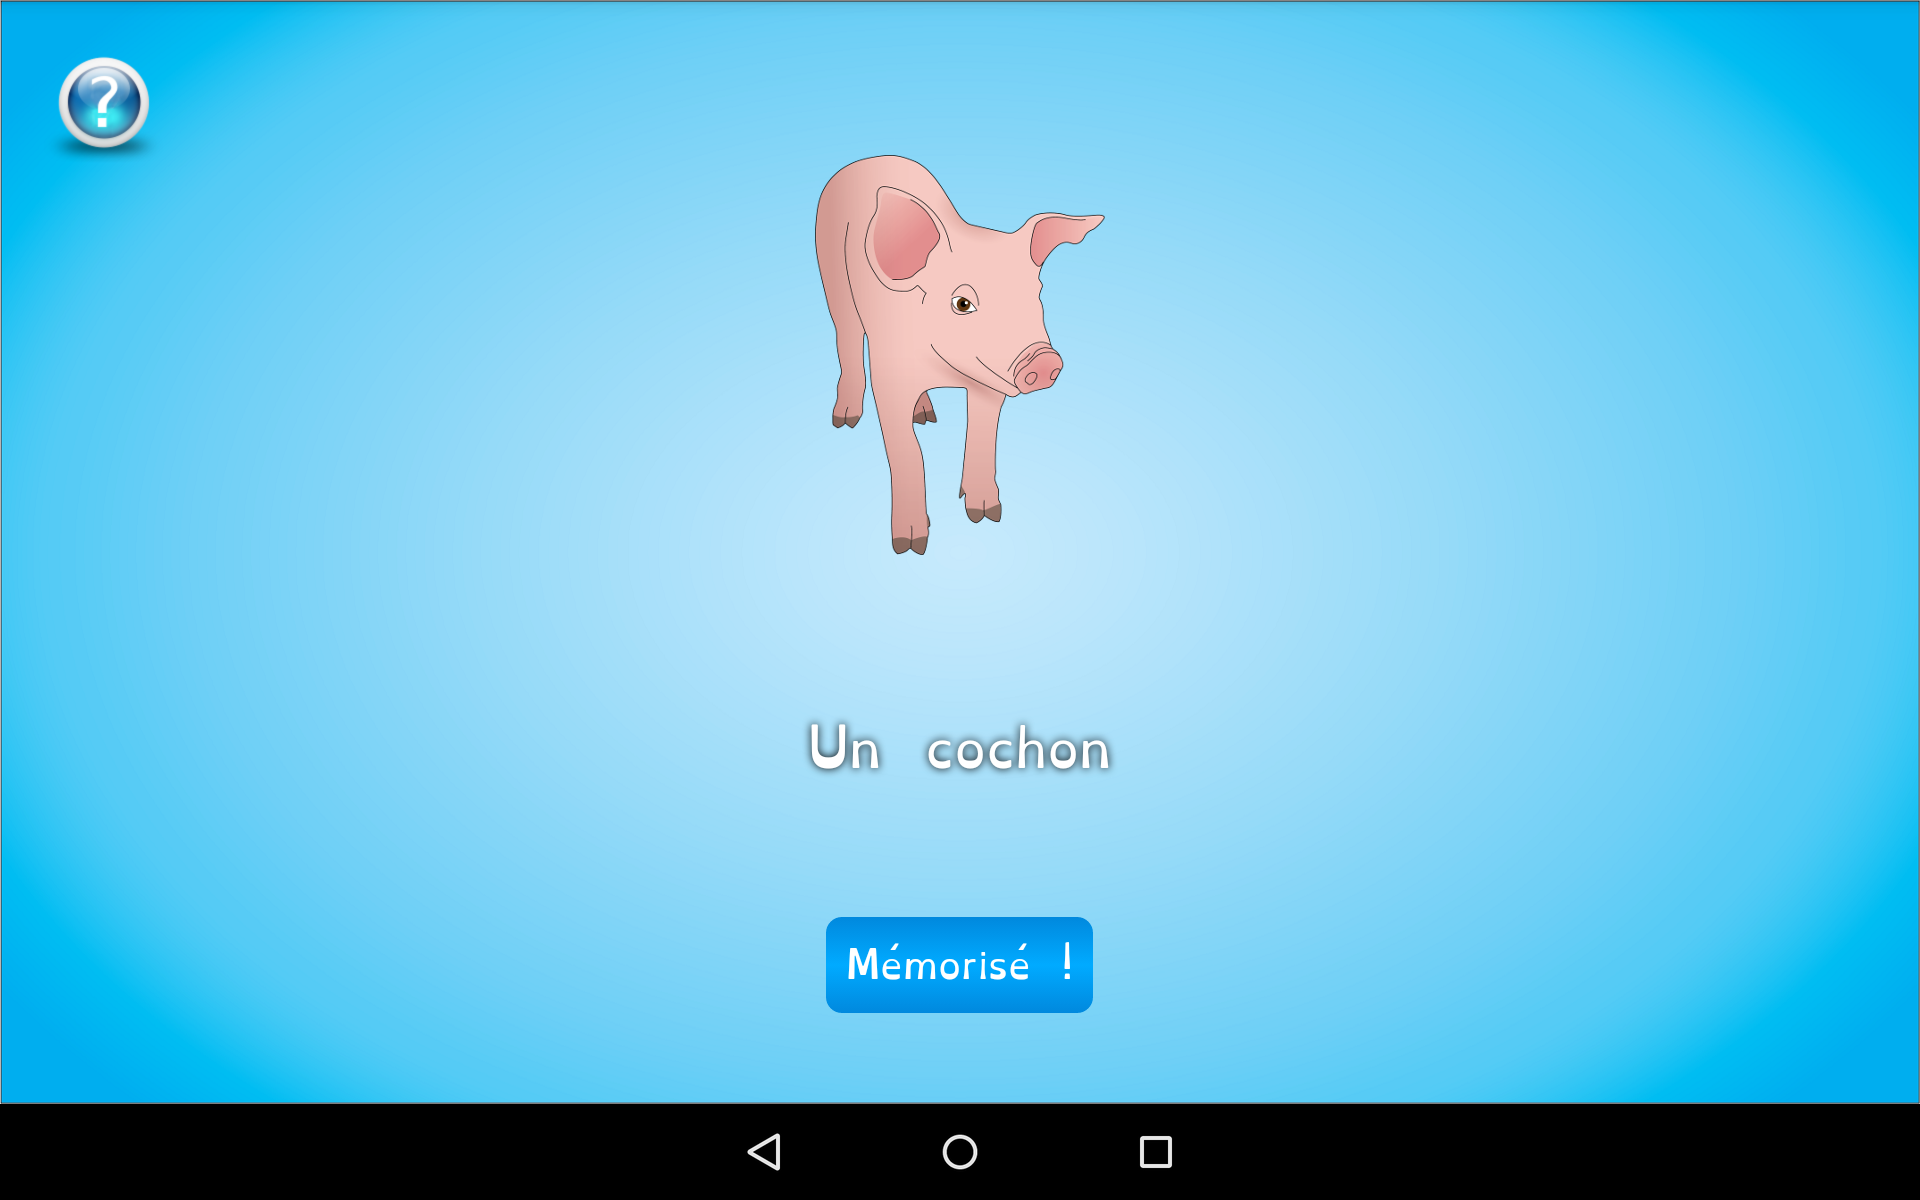
\includegraphics[width=8.5cm]{img/img-start.png}
\caption{Layout d'affichage du de l'image et du mot}
\label{imgS}
\end{subfigure}
~
\begin{subfigure}[t]{8.5cm}
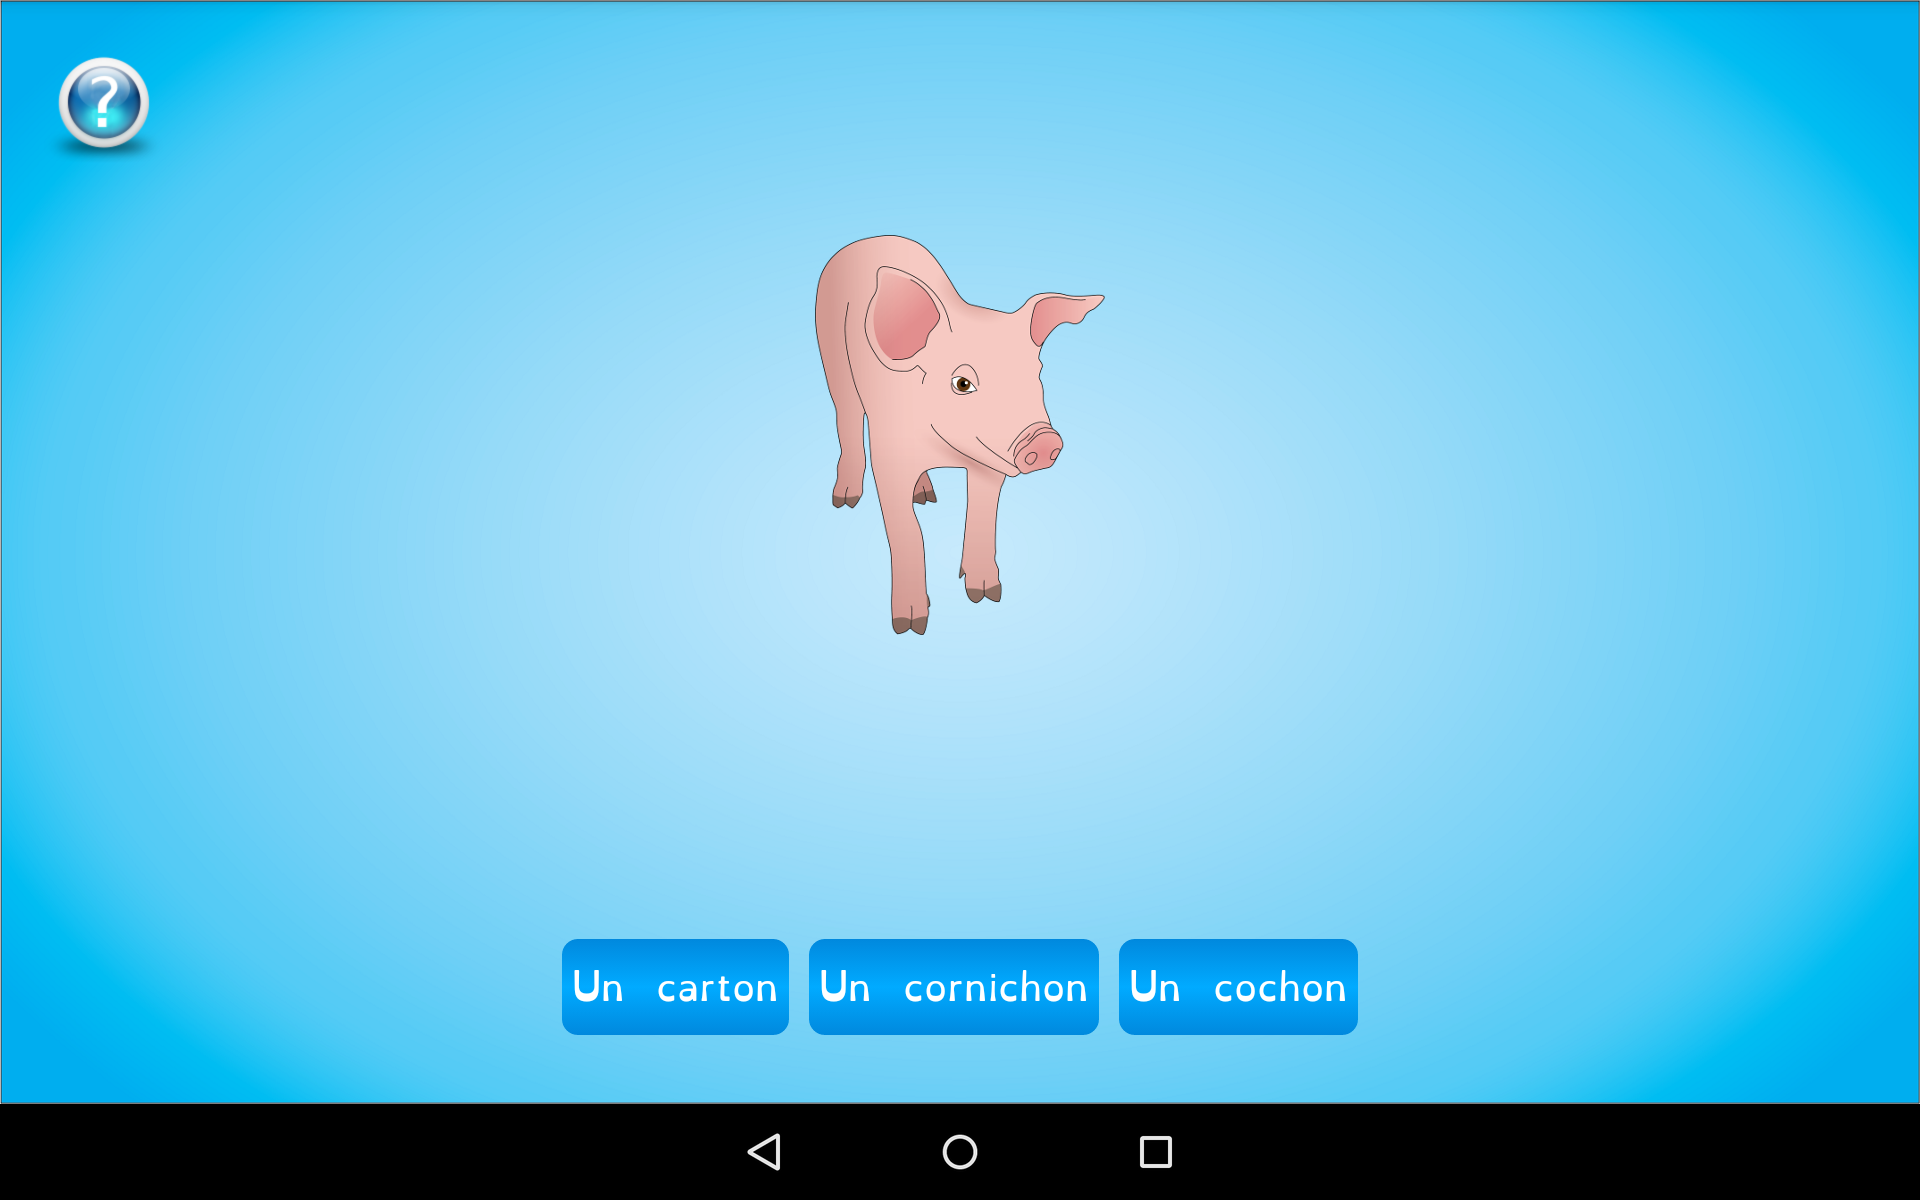
\includegraphics[width=8.5cm]{img/img-choix.png}
\caption{Layout de choix entre les mots}
\label{imgF}
\end{subfigure}
\caption{Layouts de l'exercice \textit{Imagerie}}
\end{figure}

Concernant le fonctionnement de l'exercice en lui-même, celui-ci a été défini dans la classe java correspondant à l'activité. Tout d'abord, il faut savoir qu'en Android, les chaînes de caractères sont stockées dans un fichier \textit{strings.xml}. Les autres types de ressources sont également placées dans des dossiers spécialisés. Pour les images, ces dossiers s'appellent \textit{drawable}. Il existe plusieurs dossiers \textit{drawable}, stockant respectivement les même images, mais correspondant toutefois à une résolution d'écran différente. Pour accéder à l'une des ressources, que ce soit chaîne de caractères, image, ou autre, le nom permettant de l'identifier est requis. Sachant cela, j'ai utilisé une nomenclature permettant de lier facilement les mots et les images leur correspondant. L'image et le mot correct qui lui est attribué portent le même nom. Celui-ci est de type \textit{img\_XX}, où \textit{XX} correspond au numéro identifiant le couple. Les deux réponses incorrectes sont quand à elles nommées dans le fichiers \textit{strings.xml} \textit{img\_XX\_1} et \textit{img\_XX\_2}.\\

Le principe utilisé pour \textit{Imagerie} est simple. L'image affichée est choisie au hasard parmi les possibilités. Pour ce faire, je génère un nombre random compris entre 0 et le nombre d'images - 1 (20 dans le cas présent). Ce nombre est alors concaténé à une chaîne de caractères afin de former le nom de la ressource que le système doit aller rechercher. Étant donné que l'exercice est constitué de 10 images à la suite, je vérifie également que la ressource n'a pas déjà été utilisée lors de la série (valable pour tous les exercices). À partir de cette chaîne de caractères, l'image et le mot peuvent être chargés et affichés sur le premier layout. Pour le second layout, celui proposant les choix, l'ordre d'affichage des réponses dans les boutons est également défini au hasard. J'applique alors un random entre 0 et 2. L'ordre de sortie des nombres me donne l'ordre d'affichage des réponses. Pour que le système puisse aller rechercher les mauvaises réponses, je concatène la chaîne précédente avec le numéro attribué à la réponse.\\

 %Une fois les layouts définis, la première étape a été d'afficher une image précise avec son mot, de la valider, puis de passer au choix multiple pour cette image. Dans l'arborescence d'Android, les images sont stockées dans des répertoires appelés \textit{drawable}, et les chaînes de caractères dans un fichier nommé \textit{strings.xml}. Sachant cela, et afin de me faciliter la tâche, j'ai donné à l'image et au mot le même nom. Ce nom est de type \textit{img\_XX} où \textit{XX} correspond au numéro identifiant l'image. Dans le cas du niveau 1, j'ai pour ce TFE créé 21 images. Les numéros s'étendent donc de 0 à 20. Pour les deux réponses incorrectes, je les ai respectivement nommées \textit{img\_XX\_1} et \textit{img\_XX\_2}. Le choix de cette nomenclature s'expliquera dans le paragraphe suivant. En ce qui concerne l'étape dont je parle actuellement, elle a été réalisée avec une seule image, hardcodée.\\
 
%Par après, j'ai rajouté le choix de l'image au hasard, ainsi que l'affichage de l'ordre des réponses au hasard. C'est ici que le choix de la nomenclature prend tout son sens. En effet, le \textit{XX} précédemment cité. Celui-ci est choisi au hasard dans l'intervalle spécifié, pour ensuite être concaténé afin de former la chaîne de caractère correspondant aux identifiants de l'image et du mot. Enfin, j'ai implémenté une boucle afin que l'exercice soit une série de 10, tout en m'assurant que les mots ne puissent pas être deux fois identiques dans cette série en mémorisant ceux piochés précédemment.\\

Concernant les réponses proposées pour l'exercice, il m'a fallu trouver un système permettant à l'enfant qui joue de savoir clairement s'il s'est trompé où s'il a réussi. J'ai pour ce faire mis en place un \textit{toast} qui apparaît lorsqu'on clique sur un des boutons de réponse. En Android, un \textit{toast} est une sorte de notification qui se surimprime sur l'écran pendant un temps défini. Le plus souvent, il s'agit d'un message simple. Parfois, on y retrouve une image, pour ce faire, un layout spécifique est créé pour le \textit{toast}. Je voulais mettre en place un toast avec une image et un texte : "V" et "Bien joué !" pour la bonne réponse (Fig. \ref{toastOk}), "X" et "Essaye encore !" pour la mauvaise (Fig. \ref{toastKo}). J'ai donc créé le layout nécessaire, utilisable dans les deux cas, car je passe l'identifiant de l'image et le message en paramètre à l'aide d'une fonction. En fonction du type de réponse, j'assigne au bouton correspondant l'action d'affichage du \textit{toast} "réussi" ou "perdu". Par la suite, j'ai fait de ce \textit{toast} une fonction utilisable dans les différentes \textit{activités} qui composent mon application.\\

\begin{figure}[H]
\begin{subfigure}[t]{8.5cm}
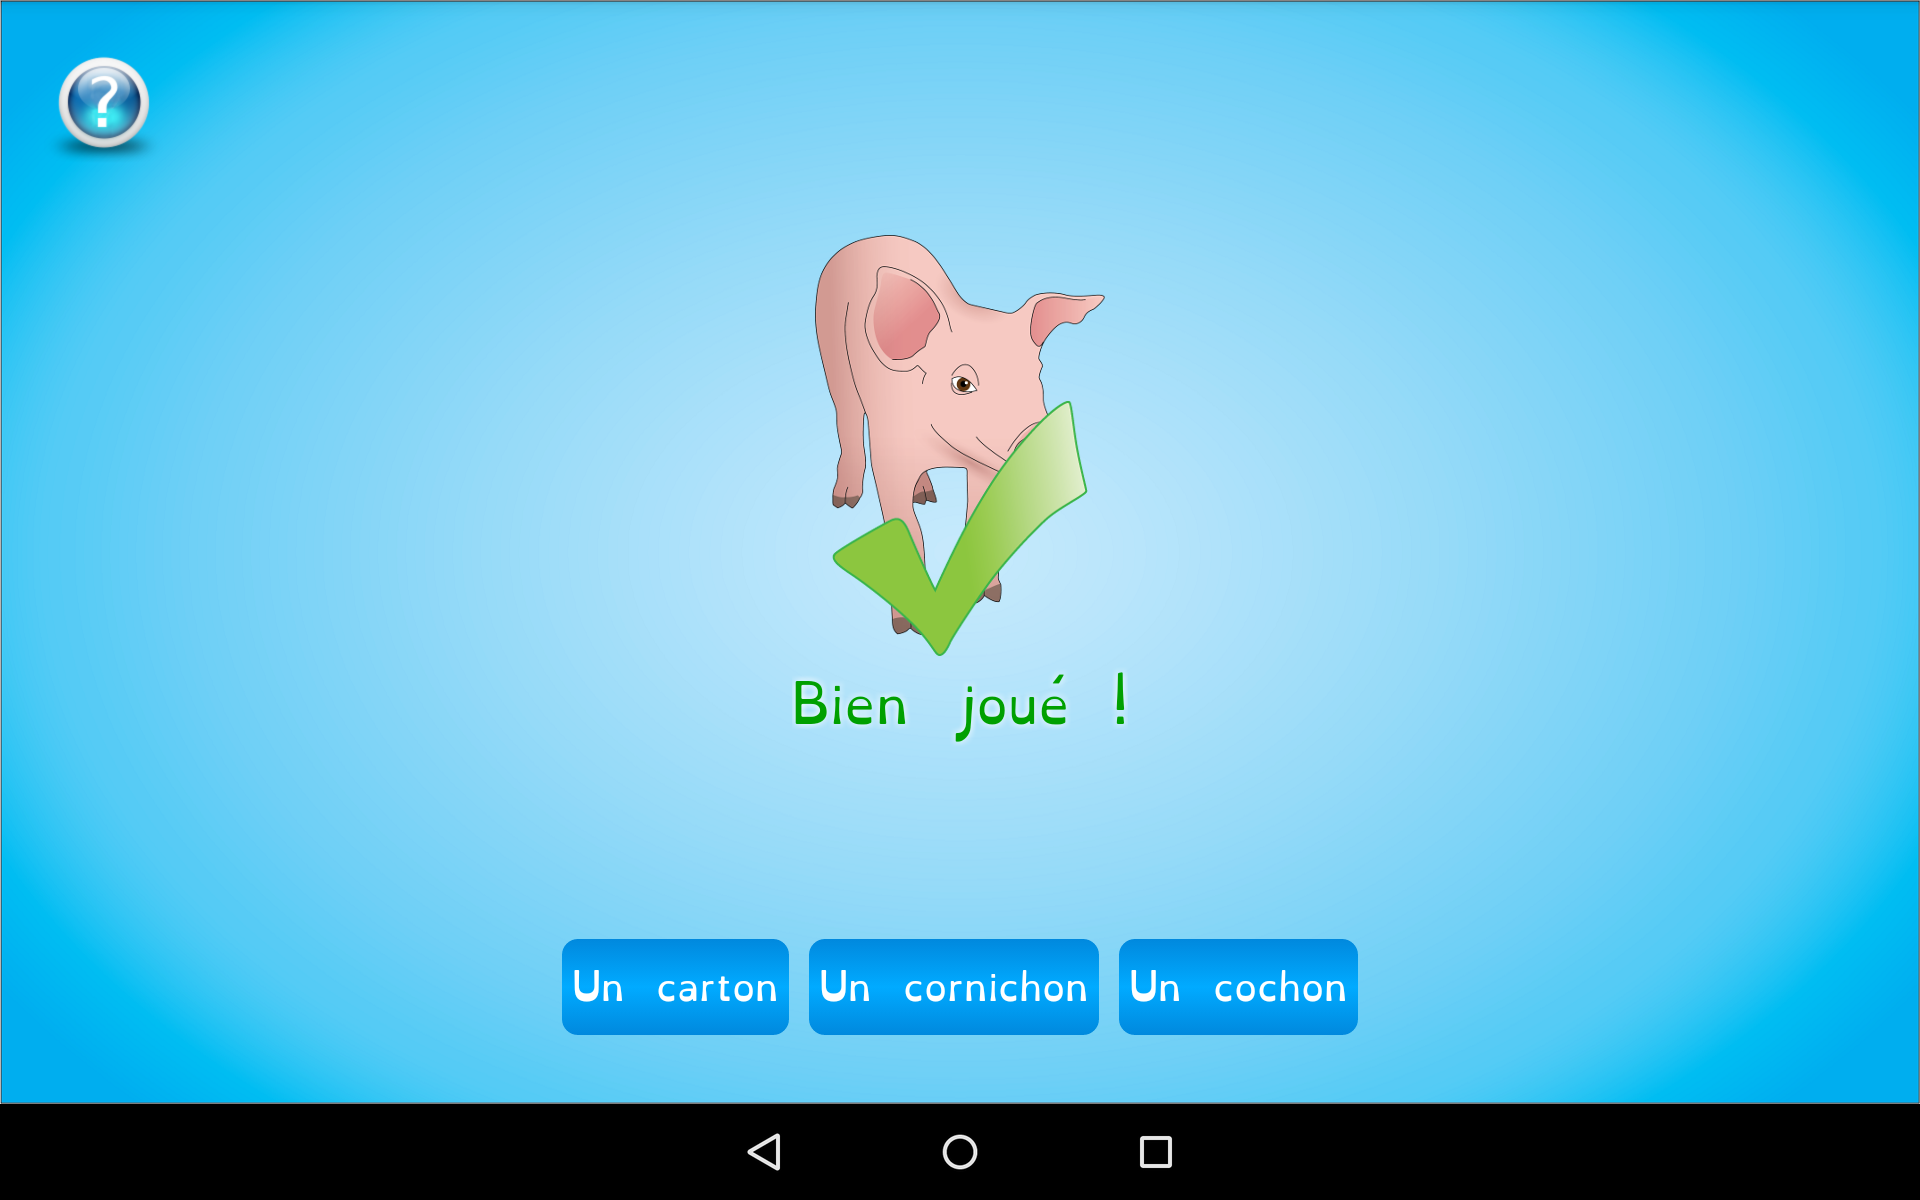
\includegraphics[width=8.5cm]{img/img-ok.png}
\caption{Affichage du \textit{toast} de bonne réponse}
\label{toastOk}
\end{subfigure}
~
\begin{subfigure}[t]{8.5cm}
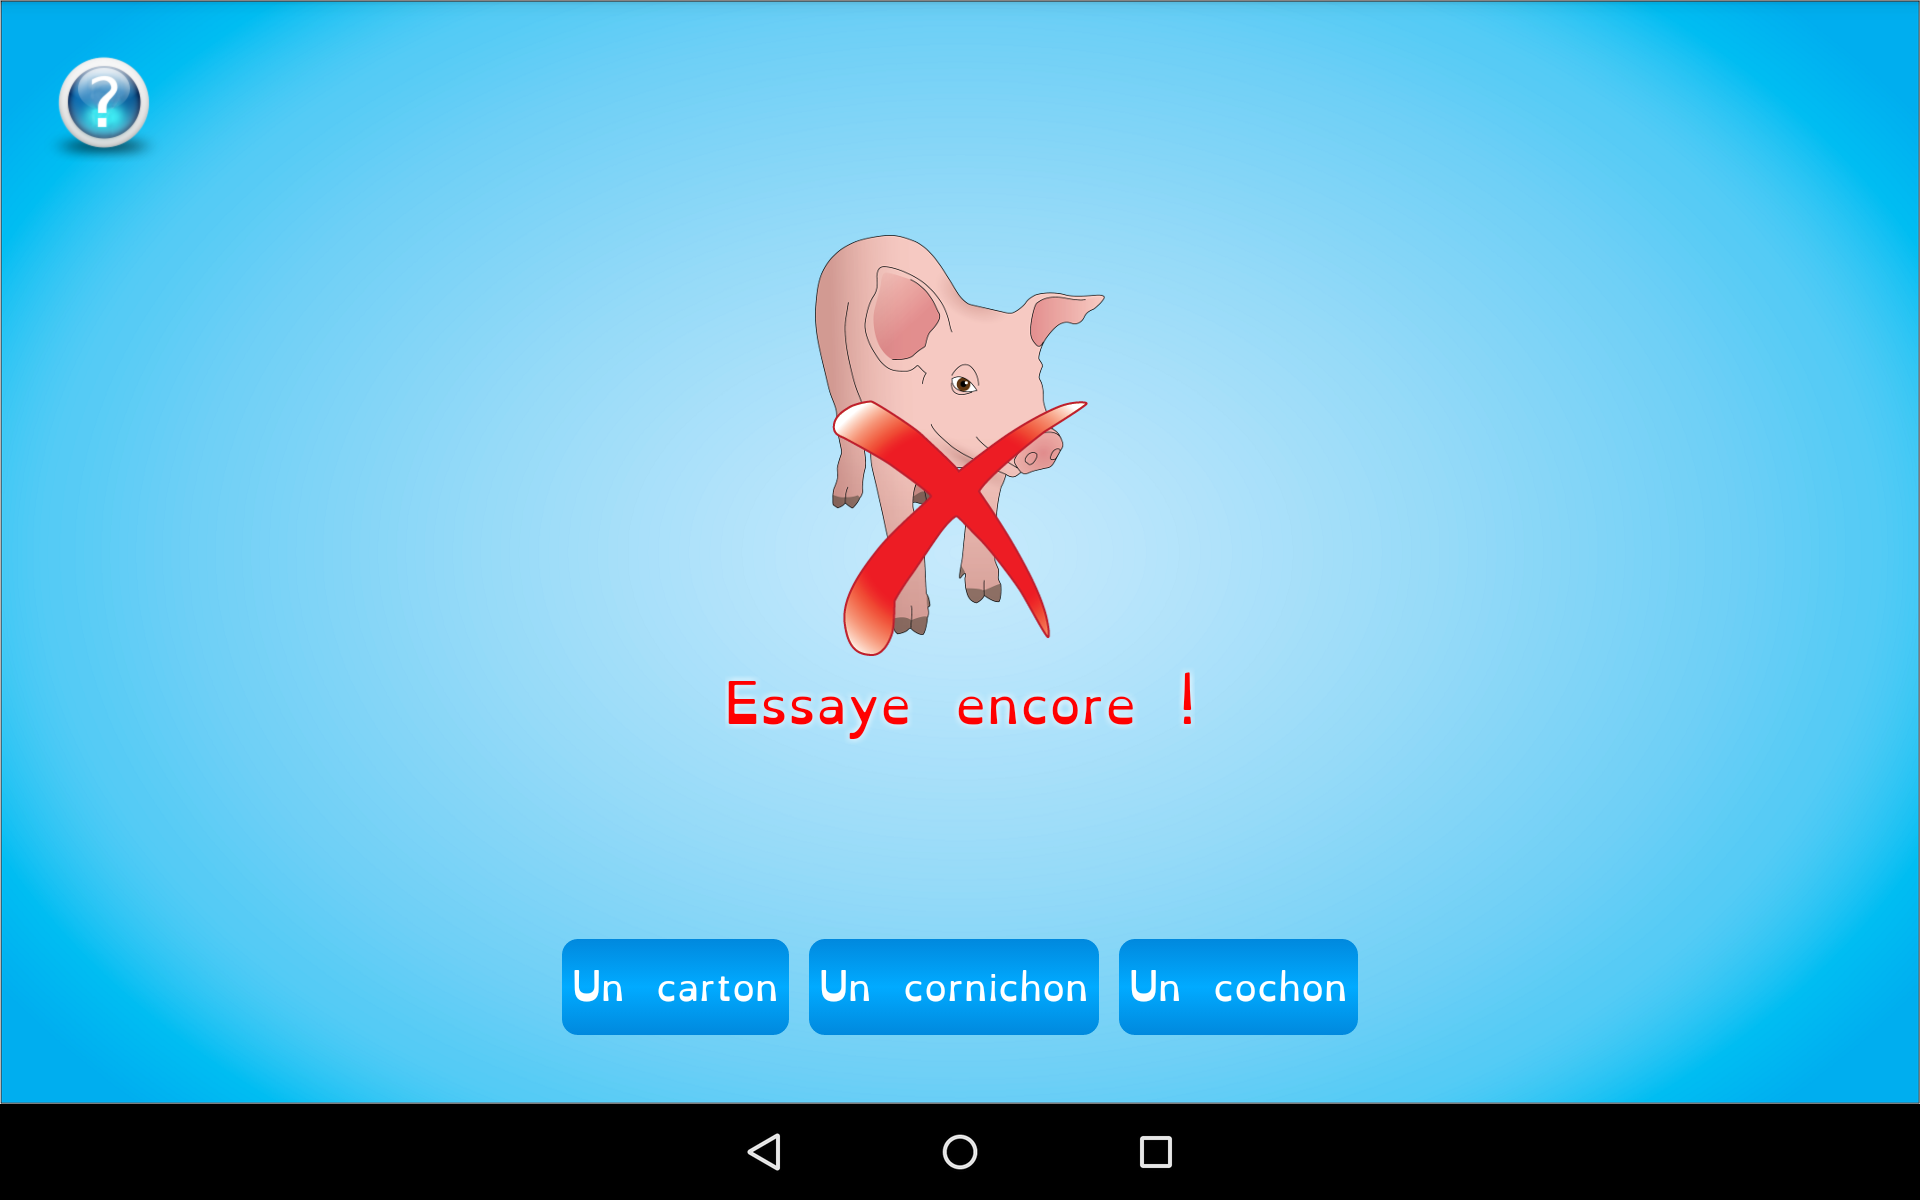
\includegraphics[width=8.5cm]{img/img-ko.png}
\caption{Affichage du \textit{toast} de mauvaise réponse}
\label{toastKo}
\end{subfigure}
\caption{Affichage des \textit{toasts}}
\end{figure}

L'exercice \textit{Imagerie} n'a pas été trop difficile à mettre en place. Une fois la logique définie, j'ai aisément pu implémenter les fonctions nécessaires. Toutefois, il s'agissait du premier exercice, j'ai donc du appréhender certaines notions. J'ai par exemple appris à lier une image ou une chaîne de caractères à un élément du layout xml à l'aide du code java afin de pouvoir modifier ce dernier.

\subsection{L'exercice \textit{Lecture flash}}
L'exercice \textit{Lecture flash} est le deuxième que j'ai mis en place pour l'application. Comme pour l'exercice précédent, j'ai d'abord commencé par le premier niveau de difficulté. Dans le cas présent, la difficulté entre les niveaux dépendra principalement de la vitesse de lecture. Pour ce premier niveau, j'ai choisi de laisser la possibilité d'afficher le mot pendant 20 secondes.\\

Les mots utilisés pour cet exercice n'ont pas été choisis au hasard. En effet, selon les conseils de Laurence Henrion et comme prévu dans le cahier des charges, j'utilise le VOB (Vocabulaire Orthographique de Base). Pour rappel, il s'agit d'une liste de vocabulaire que les enfants doivent maîtriser à la fin de chaque cycle. Dans le cadre de l'application, j'utilise le VOB du degré inférieur, qui correspond aux mots devant être connus en fin de deuxième primaire (cf. annexe \ref{listeVob}). J'ai donc recopié les 480 mots constituant le VOB du cycle inférieur dans le fichier \textit{strings.xml}. Comme précédemment, afin de faciliter le choix des mots de manière aléatoire, les noms sont identiques et différenciés par un nombre. La nomenclature de ceux-ci est \textit{str\_XXX}. \\

Pour l'interface graphique de cet exercice, il me fallait 3 layouts :
\begin{itemize}
\item un premier lors du démarrage, afin de choisir le nombre de secondes d'affichage des mots (Fig. \ref{fl1}),
\item un deuxième pour l'affichage du mot en lui-même. Très simple car il est constitué d'un seul élément (Fig. \ref{fl2}),
\item Un troisième et dernier avec un champ texte éditable et un bouton de vérification, qui est chargé une fois que le temps d'affichage du mot est écoulé (Fig. \ref{fl3}).\\
\end{itemize}

\begin{figure}[H]
\begin{subfigure}[t]{8.5cm}
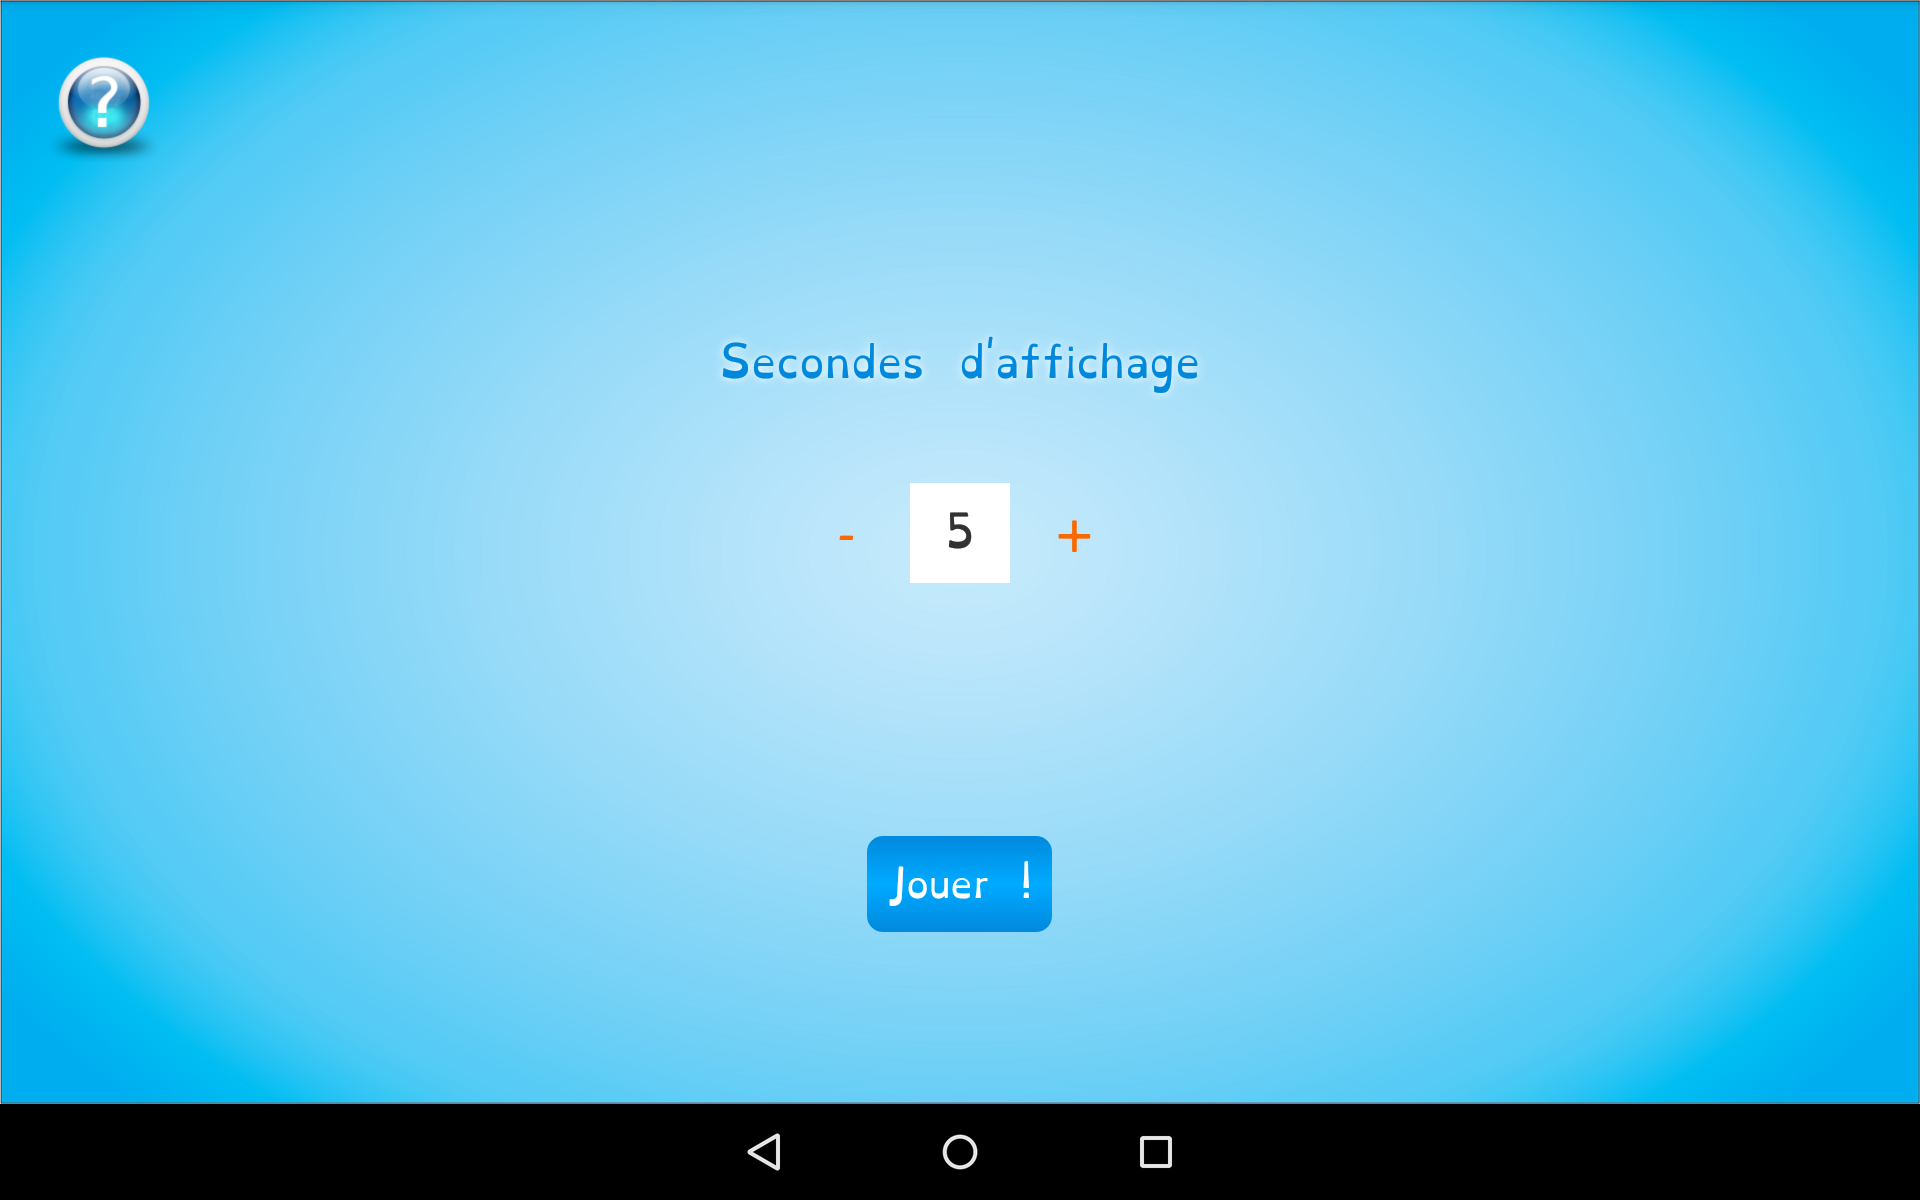
\includegraphics[width=8.5cm]{img/flash-pick.png}
\caption{Layout de choix de la durée d'affichage}
\label{fl1}
\end{subfigure}
~
\begin{subfigure}[t]{8.5cm}
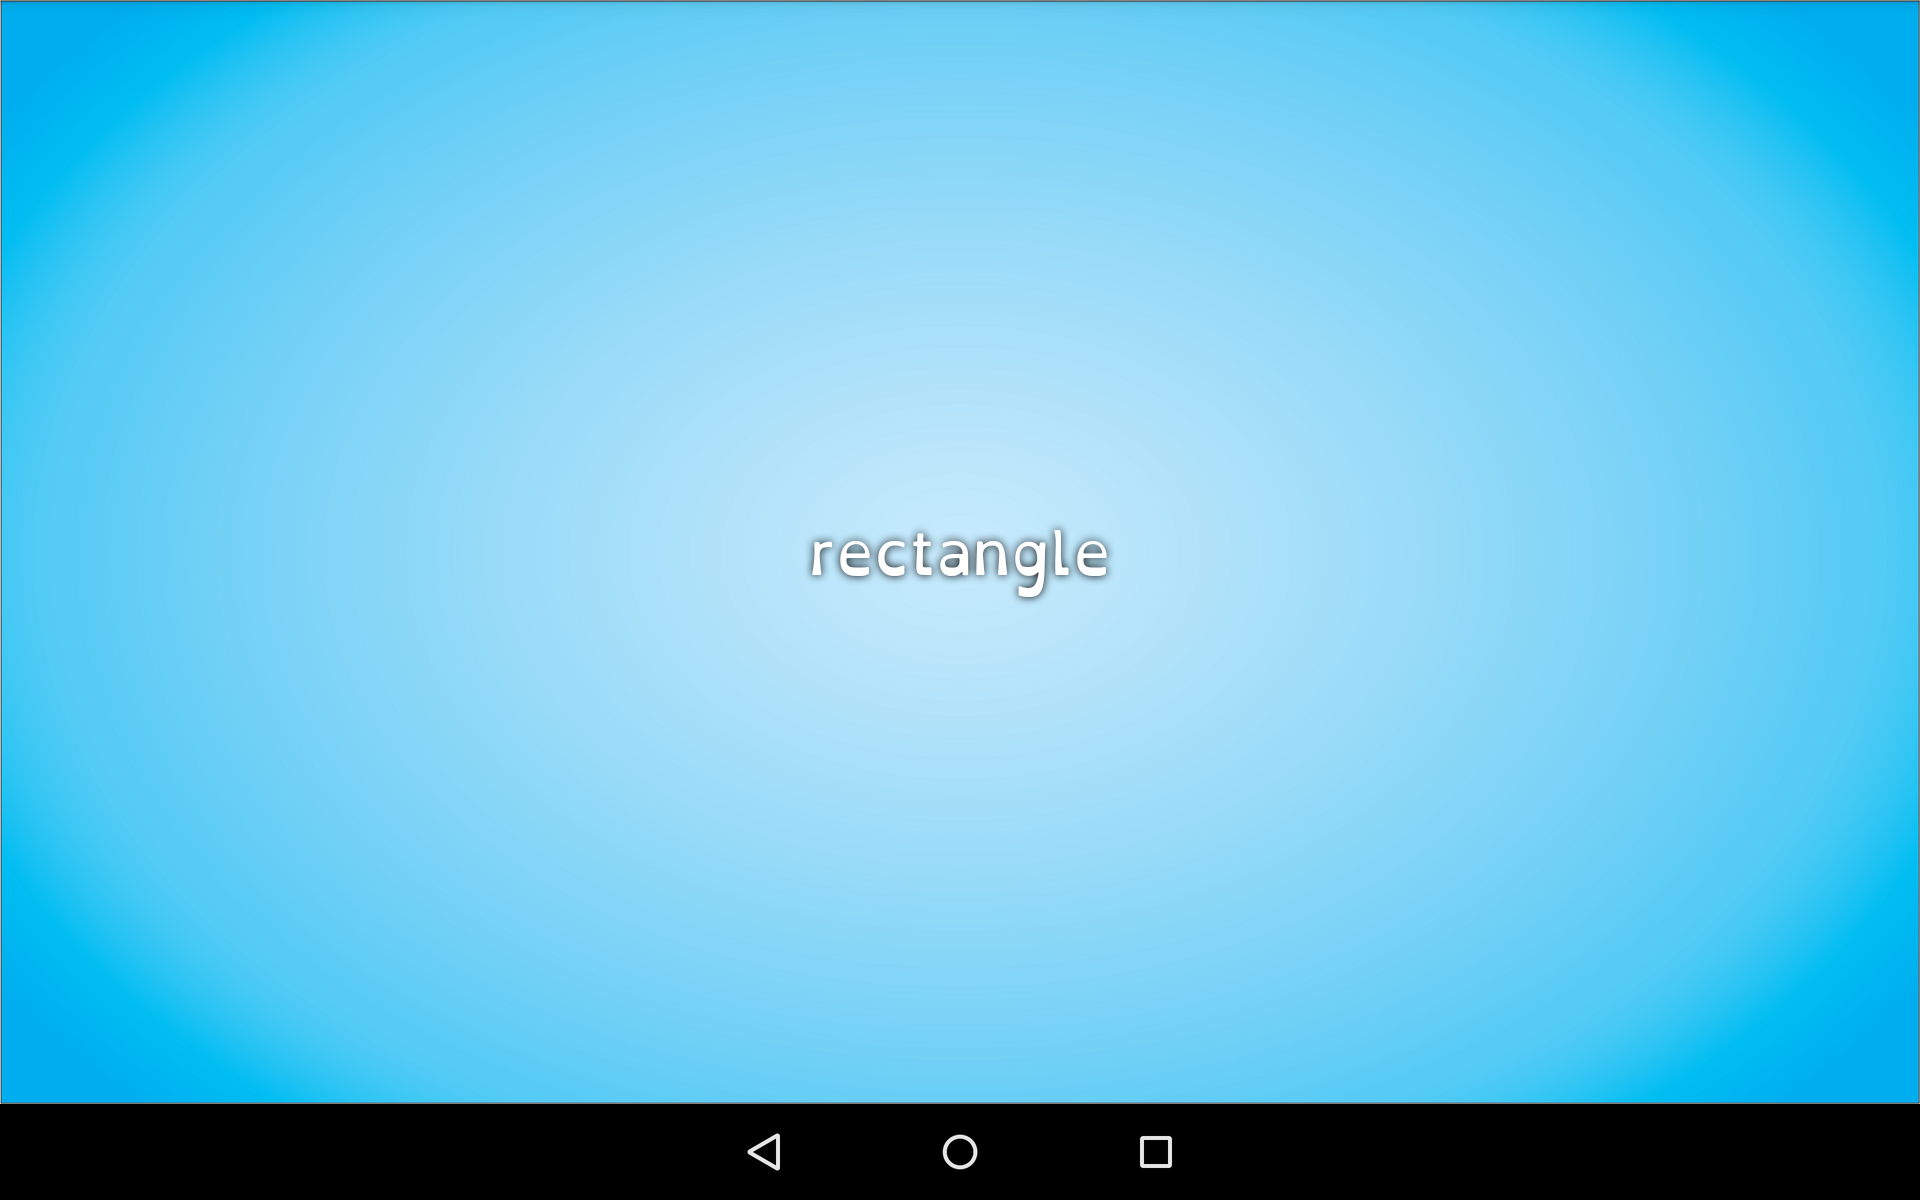
\includegraphics[width=8.5cm]{img/flash-aff.png}
\caption{Layout d'affichage du mot}
\label{fl2}
\end{subfigure}
~
\begin{subfigure}[t]{8.5cm}
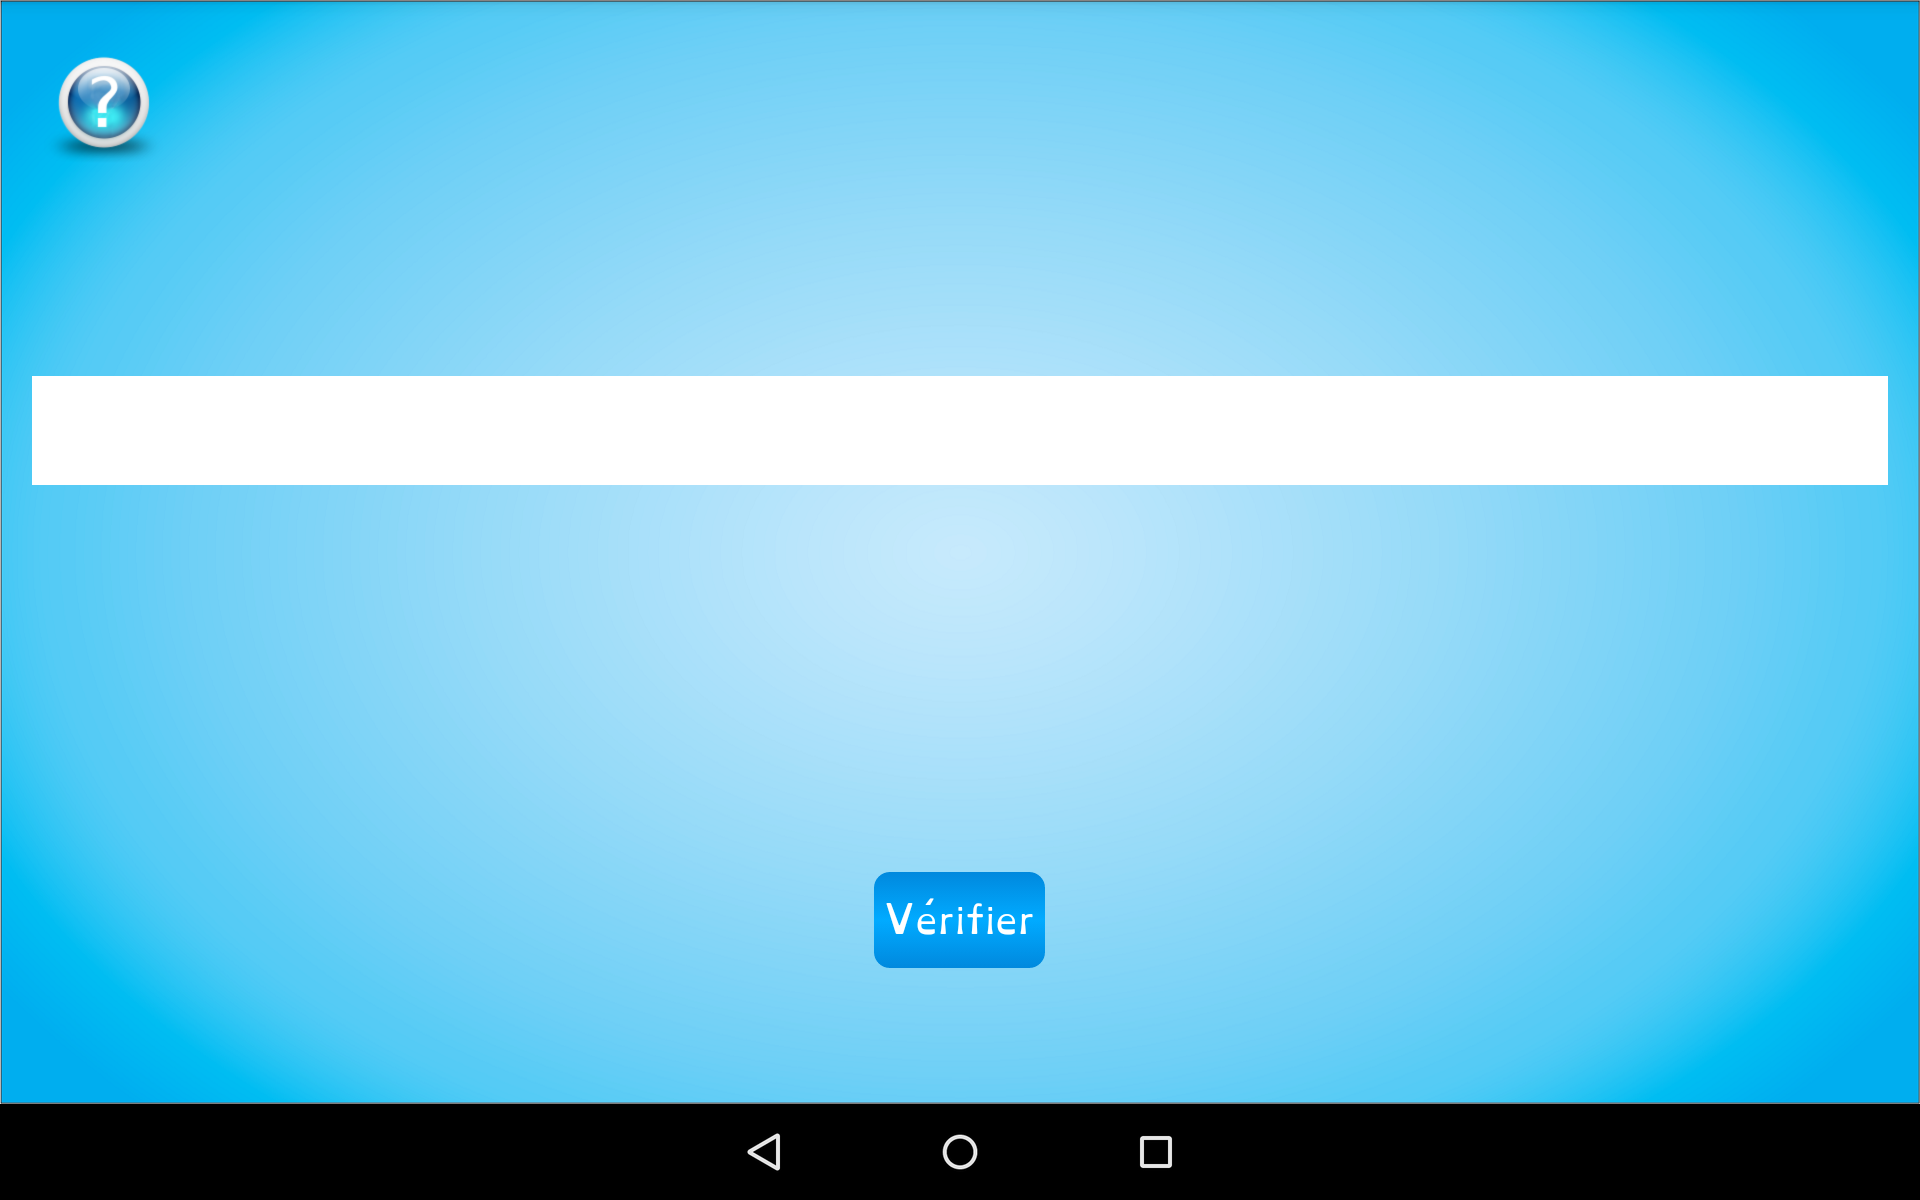
\includegraphics[width=8.5cm]{img/flash-verif.png}
\caption{Layout avec le champ pour la vérification du mot}
\label{fl3}
\end{subfigure}
~
\begin{subfigure}[t]{8.5cm}
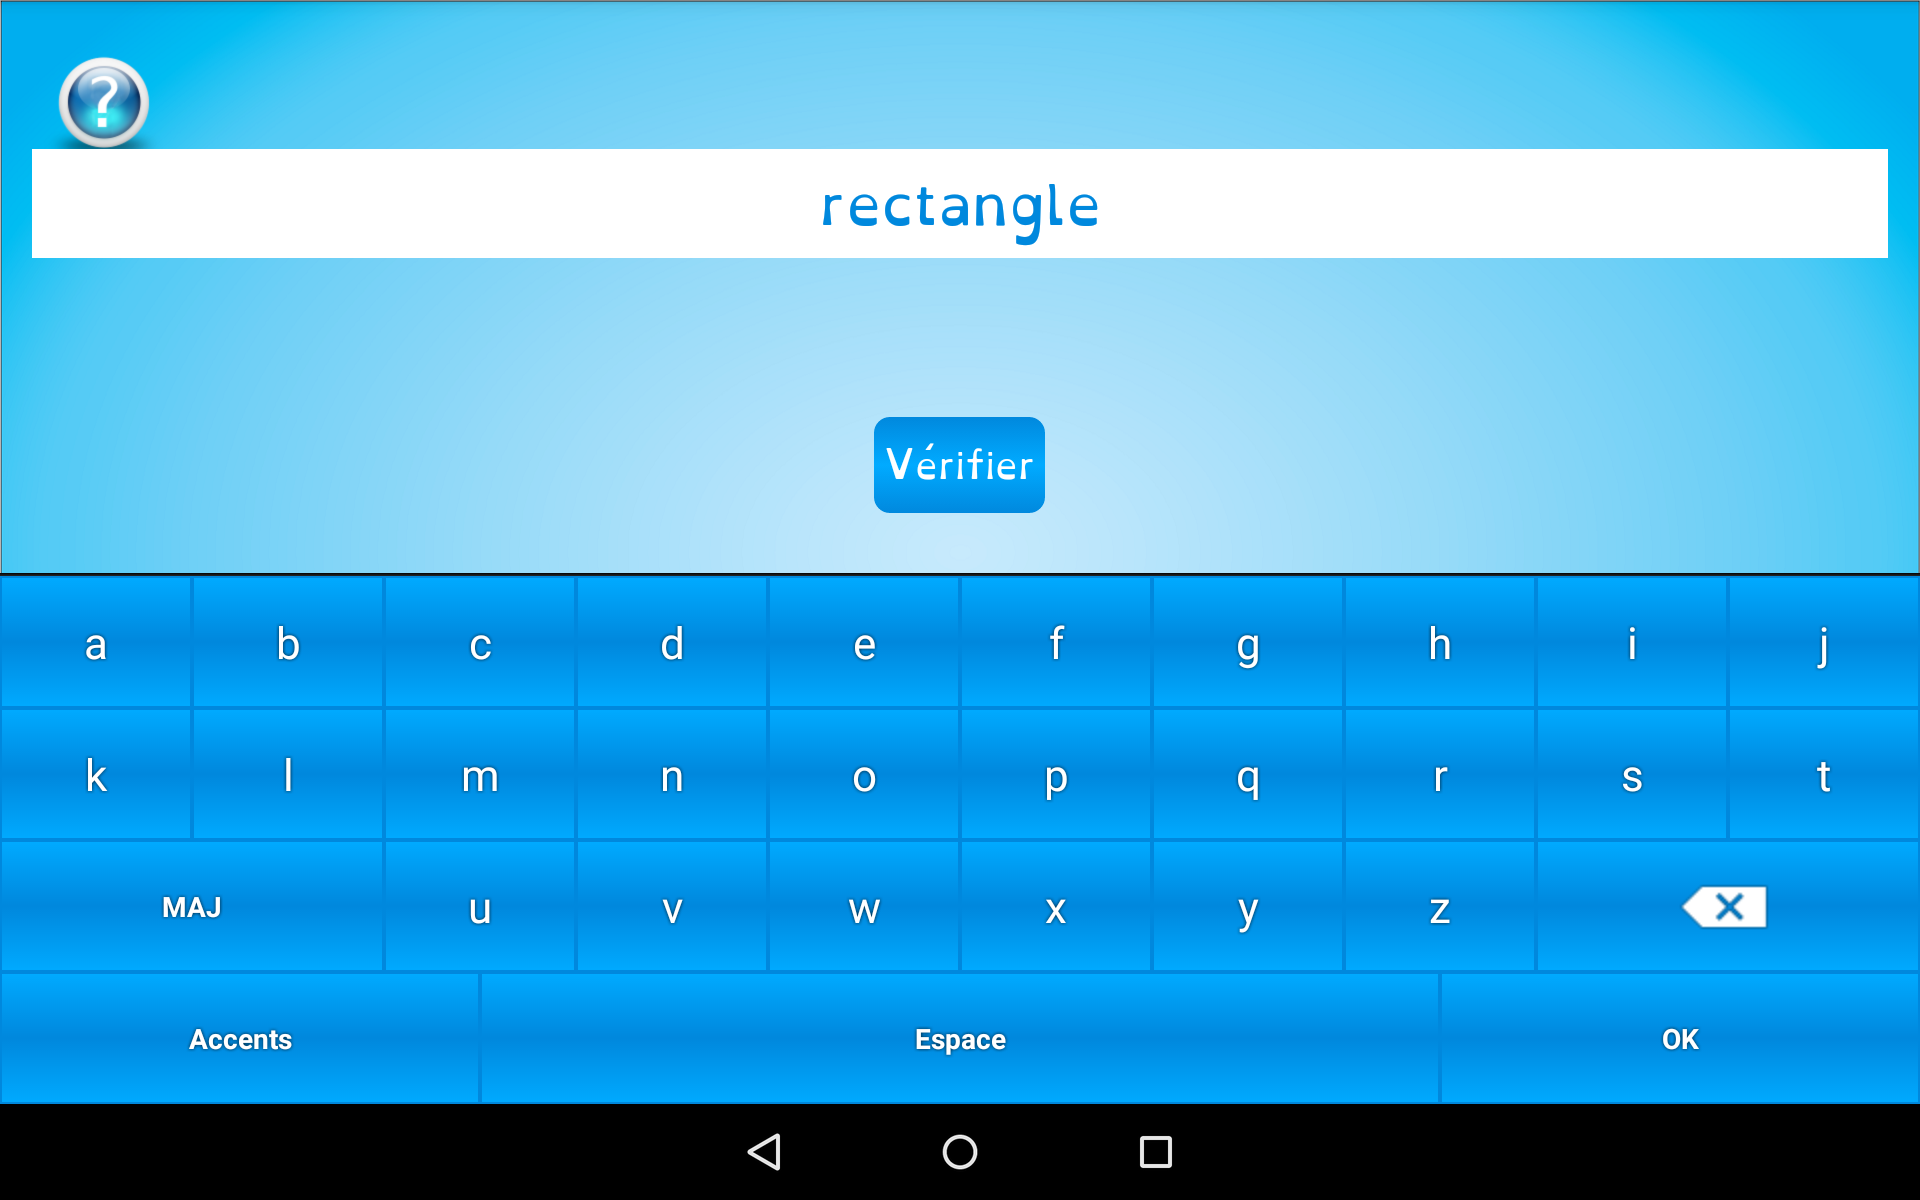
\includegraphics[width=8.5cm]{img/flash-clavier.png}
\caption{Aperçu du clavier implémenté}
\label{fl4}
\end{subfigure}
\caption{Layouts de l'exercice \textit{Lecture flash} et clavier implémenté}
\end{figure}

Du point de vue de la programmation java, j'ai créé un \textit{NumberPicker} personnalisé pour définir le temps d'affichage du mot dans le premier layout. Un \textit{NumberPicker} est un élément que l'on peut ajouter tel quel à un layout et qui permet de sélectionner un nombre dans un intervalle défini. Or, l'élément en tant que tel est très peu personnalisable. J'ai dès lors choisi de mettre en place le mien, ce qui est facile à faire. J'ai simplement aligné deux boutons avec un champ texte non éditable entre eux. J'ai assigné au bouton "-" la décrémentation du nombre dans le champ texte, et au "+" l'incrémentation.\\

La programmation concernant le fonctionnement de l'exercice en lui même est similaire à ce qui a été mis en place pour l'exercice \textit{Imagerie}. J'ai repris le principe de génération d'un nombre au hasard à concaténer par la suite une la chaîne de caractères afin d'obtenir le nom de la ressource. Ainsi, le layout d'affichage récupère la ressource, et affiche le temps pendant le temps récupéré depuis le \textit{NumberPicker} personnalisé. Le layout de vérification de l'écriture du mot à quand à lui en mémoire le mot précédemment affiché, et le compare avec ce qui est entré dans le champ texte par l'enfant. Ce dernier layout dispose également d'un bouton caché. Celui-ci s'affiche après deux erreurs de la part de l'enfant et lui propose de relire le mot.\\

%La suite de la programmation s'est déroulée de manière fluide également : l'affichage du mot le temps voulu (celui-ci récupéré du \textit{NumberPicker} codé au layout précédent), le choix au hasard du mot parmi le VOB, et la vérification du mot post-lecture. Pour le choix du mot au hasard, j'ai réutilisé le code de l'exercice \textit{Imagerie} et le modifiant pour qu'il corresponde à l'exercice.\\

Avec le développement expliqué ci-dessus, l'exercice en lui-même est fonctionnel. J'ai implémenté en supplément un clavier propre à \textit{Manabu}\label{clavier}. Ceci m'a été demandé par les enfants avec lesquels j'ai eu l'occasion de tester l'application, et notamment cet exercice (cf. point \ref{testFlash}). Ceux-ci préféraient avoir un clavier pour lequel il ne devaient pas réapprendre l'ordre des lettres, et donc un de type \textit{alphabet} plutôt qu'un \textit{azerty}. Afin de mettre en place mon propre \textit{SoftKeyboard}, je me suis inspirée du tutoriel de Martin Pennings et j'ai téléchargé le code source disponible sur la page du celui-ci\footnote{Maarten Pennings,\textit{Android development: Custom keyboard}, \url{http://www.fampennings.nl/maarten/android/09keyboard/index.htm}, consulté le 18 mai 2015}. Après avoir essayé de compléter mon code sur la base du tutoriel seul, sans grand succès, j'ai décidé d'intégrer le code source précédemment téléchargé à mon projet.\\

Enfin, le code source de Martin Pennings étant destiné à mettre en place un \textit{Softkeyboard} hexadécimal, je ne l'ai pas gardé tel quel. J'ai remplacé le seul layout fourni de base par quatre nouveau layouts composants mon clavier :
\begin{itemize}
\item un layout avec les 26 lettres de l'alphabet en minuscule (Fig. \ref{fl4}),
\item un layout avec les 26 lettres de l'alphabet en majuscule,
\item un layout avec les lettres accentuées en minuscule et la ponctuation,
\item un layout avec les lettres accentuées en majuscule et la ponctuation.
\end{itemize}
De ce fait, j'ai également modifié certaines parties du code précédemment intégré afin de l'adapter aux besoins de \textit{Manabu}.\\

La mise en place du premier niveau de l'exercice \textit{Lecture flash} en lui-même s'est donc déroulée sans encombre. Comme expliqué ci-dessus, la partie la plus ardue a été l'implémentation du clavier \textit{alphabet} à partir du code de quelqu'un d'autre.
	
\subsection{L'exercice \textit{Anagrammes}}
\textit{Anagrammes} est le troisième exercice que j'ai implémenté. C'est également durant la mise en place de celui-ci que j'ai pu faire tester l'application par des enfants (cf. point \ref{testEnfants}).\\

%Voir si je rajoute des éléments
Il s'agit d'un des deux exercices qui nécessitent le moins de layouts. En effet, je n'ai mis qu'un layout en place. Par défaut, celui-ci contient uniquement un bouton permettant de ré-écouter le mot dont il faut remettre les lettres dans l'ordre. Les autres éléments de ce layout sont ajoutés de manière programmée lors de la génération d'un nouvel anagramme.\\

Bien que mettre en place le layout ait été un jeu d'enfant, je ne peux pas dire qu'il en soit allé de même pour la programmation. Je m'y suis reprise plusieurs fois afin de parvenir à un résultat correct et le plus proche possible de ce que j'avais imaginé. Les difficultés rencontrées lors du développement de cet exercice seront expliquées par la suite, au point \ref{diff} \textit{Difficultés rencontrées}. Voici donc l'explication des actions programmées pour cet exercice.\\

Tout d'abord, j'ai repris le bout de code de l'exercice \textit{Lecture flash} servant à aller chercher une chaîne de caractères au hasard. En effet, j'utilise également le VOB pour les anagrammes. Pour le niveau 1, je limite le mot à minimum 3 et maximum 5 lettres. Les niveaux suivants augmentent bien entendu le nombre de lettres, ce qui les rend plus difficiles. Ensuite, je mélange les lettres du mot au hasard pour former l'anagramme\footnote{Un anagramme se définit un mot formé des mêmes lettres que le mot de base. Cependant, ici, je mélange toutes les lettres sans chercher à ce qu'elles forment un autre mot}.\\

Ensuite, j'ajoute au layout de nouveaux boutons. Pour être exacte, j'ajoute deux fois plus de boutons qu'il y a de lettres dans le mot. La moitié de ces boutons sont ajoutés sous formes de \textit{cases de validation}, blanches. Ceci signifie que les lettres mélangées viendront une par une se fixer sur l'un de ceux-ci pour reconstituer le mot original. La seconde moitié des boutons est évidemment réservée aux lettres dans le désordre. Une lettre correspond à un bouton. Les voyelles sont affichées sur un fond orange et les consonnes sont sur un fond vert. Ceci permet à l'enfant de différentier une première fois les lettres (Fig. \ref{ana1}).\\

\begin{figure}[H]
\begin{subfigure}[t]{8.5cm}
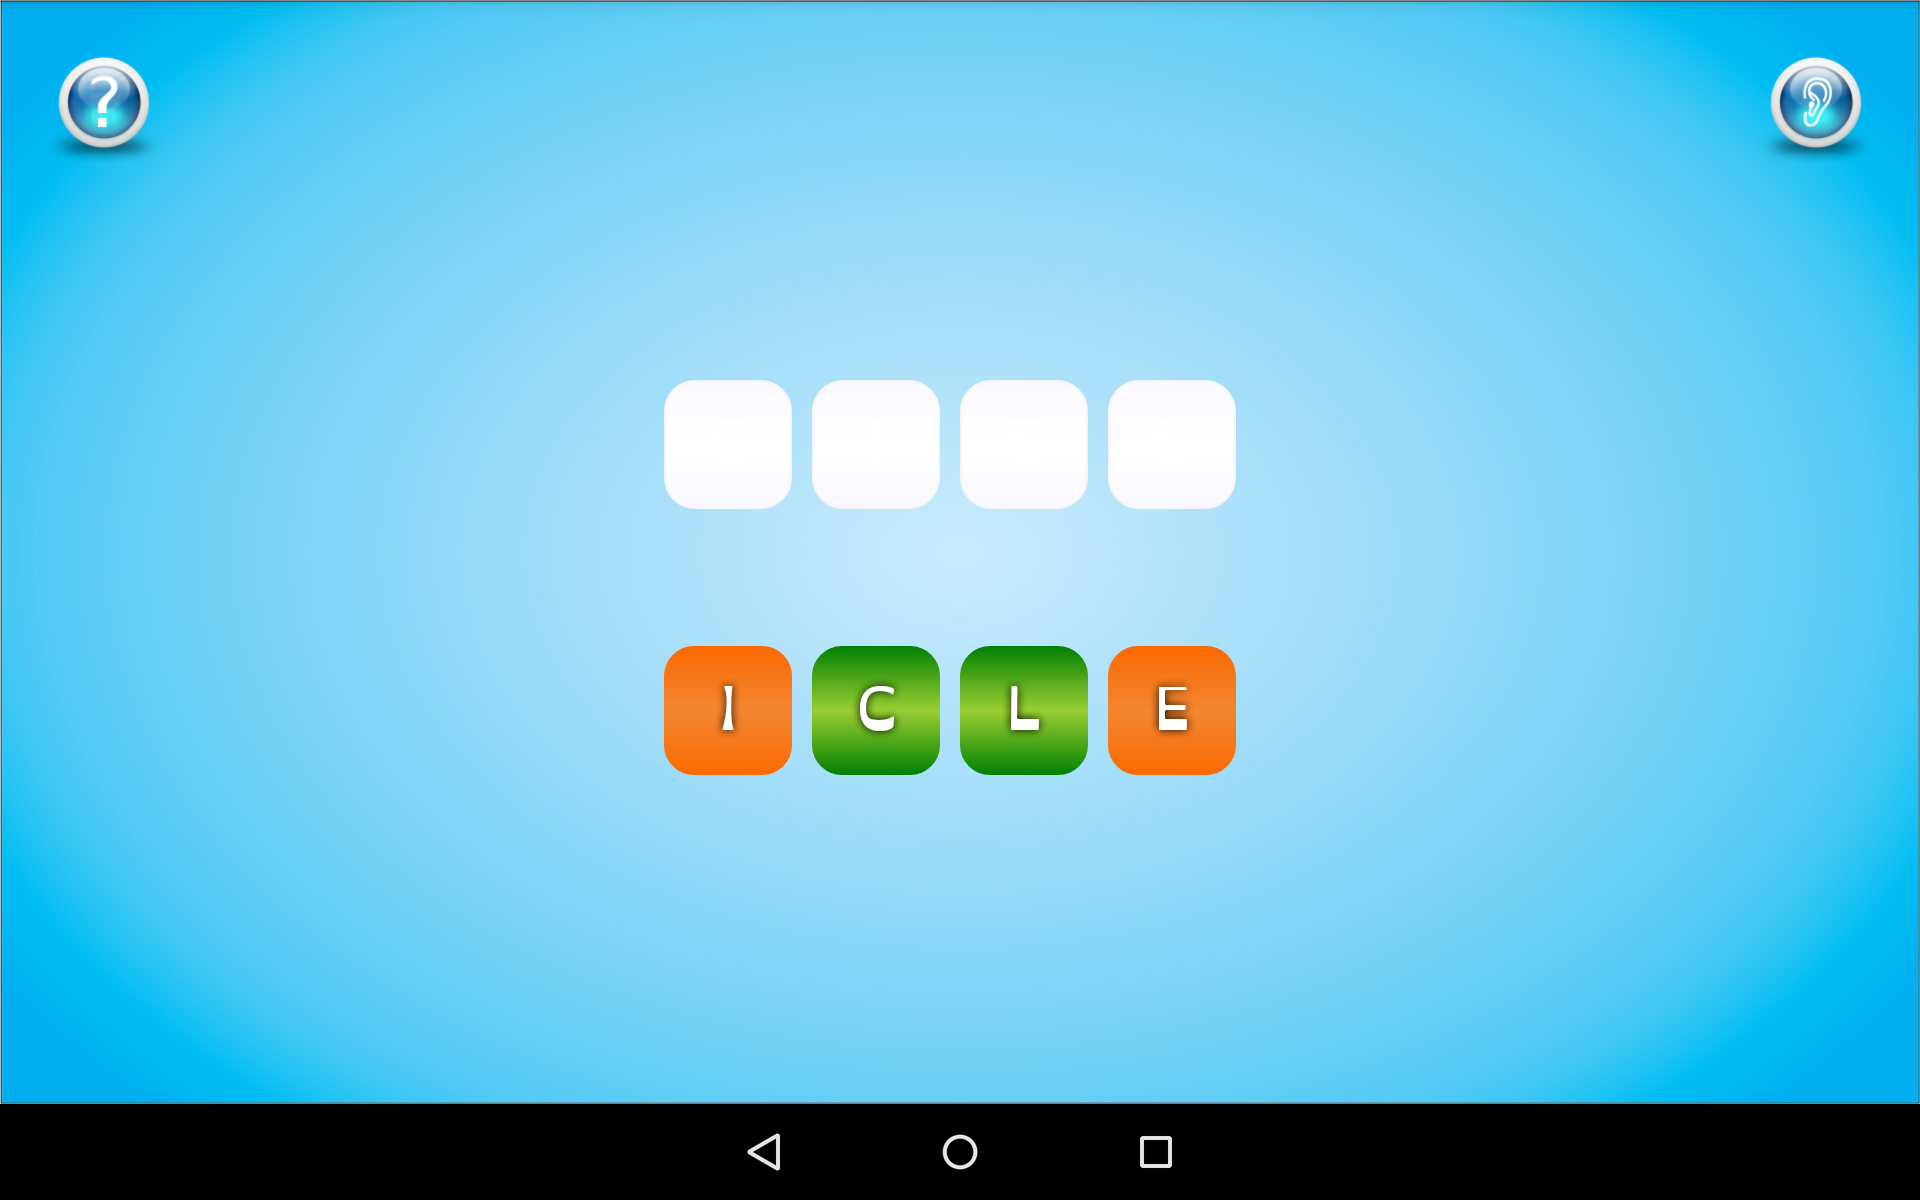
\includegraphics[width=8.5cm]{img/ana-debut.png}
\caption{Mise en place du layout de démarrage}
\label{ana1}
\end{subfigure}
~
\begin{subfigure}[t]{8.5cm}
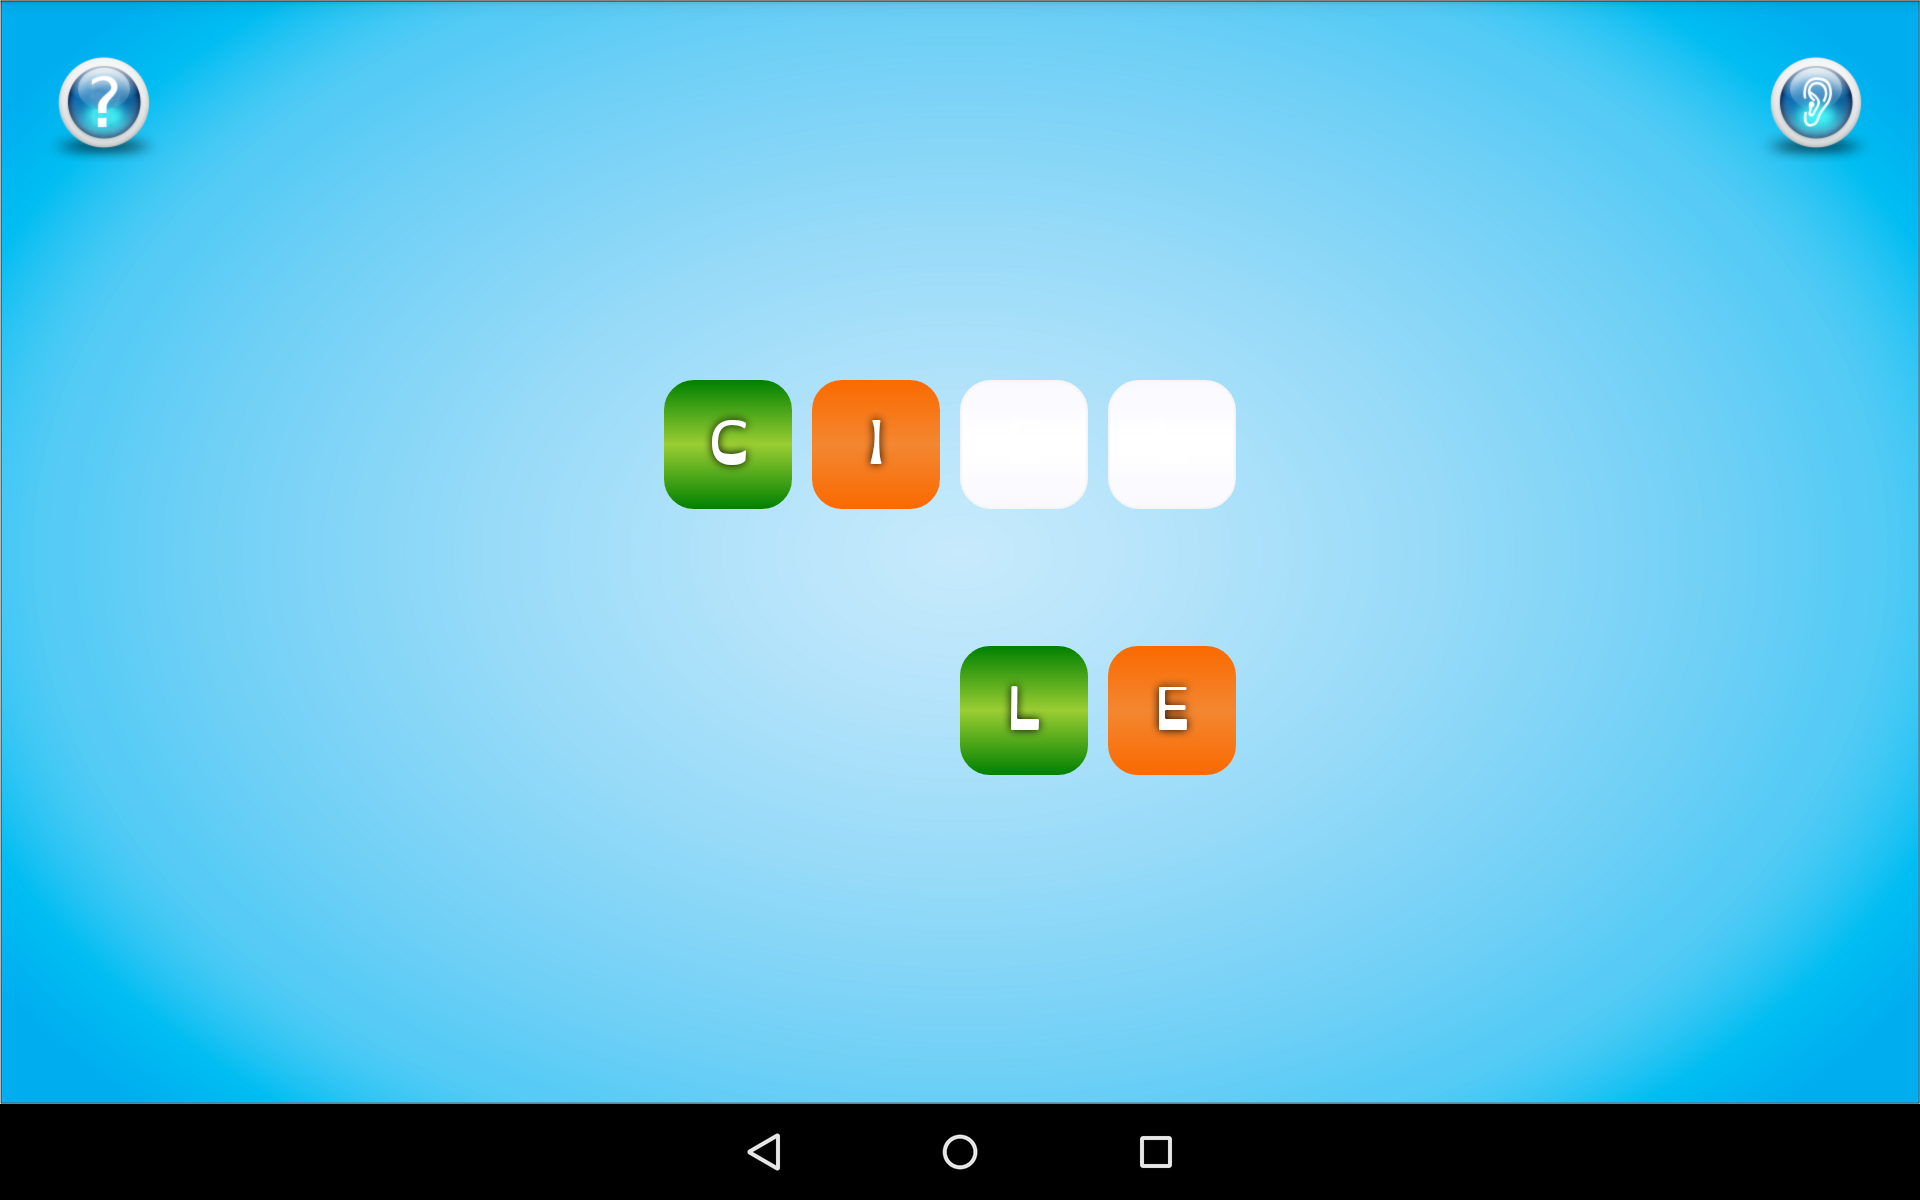
\includegraphics[width=8.5cm]{img/ana-cours.png}
\caption{Exercice en cours de réalisation}
\label{ana2}
\end{subfigure}
~
\begin{subfigure}[t]{8.5cm}
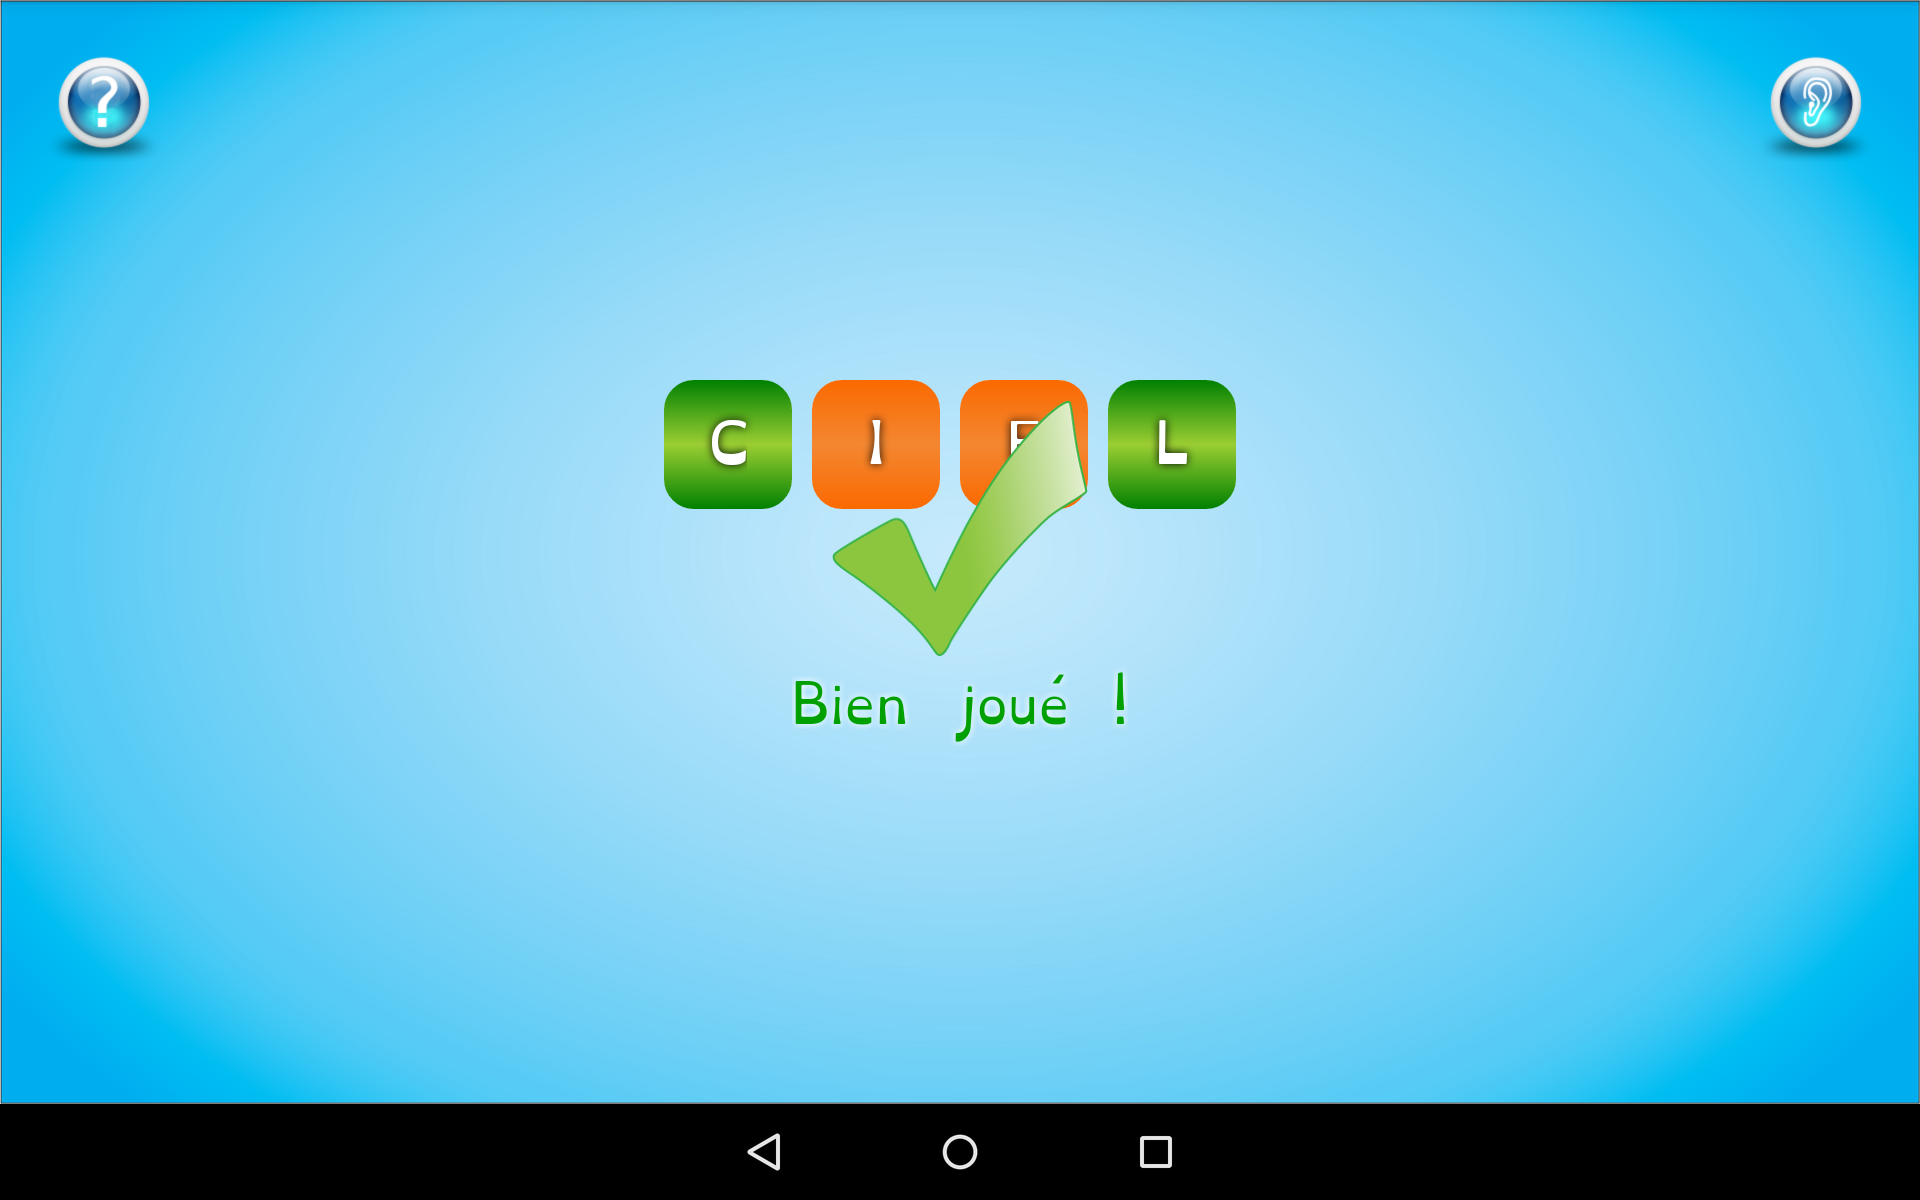
\includegraphics[width=8.5cm]{img/ana-ok.png}
\caption{Mot recontitué et validation de l'exercice}
\label{ana3}
\end{subfigure}
\caption{Déroulement de l'exercice \textit{Anagrammes}}
\end{figure}

La validation de la remise en ordre des lettres est l'étape cruciale de cet exercice. Les boutons contenant les lettres mélangées ont tous un \textit{on touch listener}. Ce dernier leur permet de suivre le mouvement du doigt qui les guidera jusqu'à la bonne \textit{case de validation}(Fig. \ref{ana2}). Afin de valider la position d'une lettre sur une de ces cases, j'ai mis en place quelques petites astuces. En premier lieu, les \textit{cases de validation} contiennent la lettre correcte qui doit s'y trouver, ainsi qu'un booléen signifiant si cette lettre a déjà été placée ou non. Les boutons des lettres à réorganiser contiennent aussi un booléen pour savoir si les enfants ont trouvé la bonne \textit{case de validation}. Lors du mouvement d'une lettre, si celle-ci se trouve au-dessus de la case qui lui correspond, la position de la lettre deviendra identique à celle de la case et le mouvement ne sera alors plus possible. Le mouvement est empêché grâce aux deux booléens ayant alors pris la valeur \textit{true}. Une fois l'anagramme complété (Fig. \ref{ana3}), le suivant sera lancé, et ainsi de suite pour 10 anagrammes.\\


D'autre part, le son est une composante importante de l'exercice. Lors du lancement de chaque nouvel anagramme, l'enregistrement du mot est joué une fois afin d'indiquer à l'enfant le mot à reconstruire. Ceci m'a été demandé par des enfants lors du test (cf. point \ref{testAna}). Un bouton leur permet également de ré-écouter le mot à tout instant. De plus, j'ai ajouté un petit extra, qui selon moi donne un peu plus de consistance et de fun à l'exercice. Lorsqu'une lettre est placée correctement sur sa case, un son est se fait entendre. Celui-ci valide l'action, et encourage l'enfant qui voit ainsi qu'il progresse.\\

Enfin, je peux confirmer que cet exercice m'a demandé plus de ressources que les deux précédents. Il a été plus chronophage également. Malgré cela, il a été très intéressant à développer, car il m'a forcé à imaginer des astuces et un algorithme plus complexe que je ne l'aurais pensé afin de parvenir à mes fins.



\subsection{L'exercice \textit{Écouter le son}}
\textit{Écouter le son} est le quatrième et dernier exercice de l'application \textit{Manabu}. Celui-ci, tout comme \textit{Anagrammes}, est composé d'un unique layout.\\

Ce layout est composé de cinq boutons. Au centre de celui-ci se trouvent trois boutons alignés verticalement. Ces boutons sont prévus pour contenir les différents mots qui serviront de choix pour trouver le son entendu. En haut à gauche un bouton permet d'ouvrir le pop-up des règles et en haut à droite du layout se trouve également le dernier bouton permettant de ré-écouter le son.\\

Pour la programmation, j'ai tout d'abord commencé par établir un algorithme sur papier avant de me lancer dans le développement proprement dit. J'ai décidé de repartir sur le principe du nombre aléatoire. Ici, le nombre aléatoire décide du son que l'enfant devra reconnaître. A partir de ce son, je retrouve les mots du VOB le contenant pour en sélectionner un. Cependant, chaque niveau demande à l'enfant de retrouver le mot contenant le son à des endroits différents. En effet, au niveau facile le son se trouve au début, au niveau moyen au milieu, et au niveau difficile n'importe où dans le mot.\\

Partant de cet énoncé, j'ai décidé d'éviter de me lancer dans des algorithmes compliqués, et de réaliser un fichier texte référentiel par niveau. Chacun des fichiers est une sorte de dictionnaire phonétique. Sur chaque ligne se trouve un code unique de type \textit{XXYYY}. Le \textit{XX} correspond au code que j'ai associé à un son\footnote{Par exemple, le son \textit{a} de arbre est associé au code \textit{AA}, le son \textit{k} dans carré, kilo, ou quelque au code \textit{KK}, etc.}, et le YYY au numéro de la chaîne de caractères, utile pour la retrouver dans \textit{strings.xml}. Dans le fichier, les codes sont classés par son (tous les \textit{a}, puis tous les \textit{au}, puis les \textit{b}, et ainsi de suite). Selon le niveau sélectionné, au démarrage de l'exercice, le fichier correspondant à celui-ci est chargé en mémoire dans une \textit{ArrayList} code par code. Un index de cette liste est créé afin de ne pas avoir à en parcourir l'entièreté lors de la recherche d'un mot pour un son précis. Cet index est un tableau d'entiers de la taille du nombre de sons possibles. Chaque case de celui-ci contient la position du début d'un type de son dans l'\textit{ArrayList}, la position dans le tableau elle-même équivalant à l'identifiant du son.\\

Les événements programmés se déroulent dans un ordre défini. Tout d'abord, un nombre \textit{random} est généré, avec pour maximum, le nombre de sons existants, puis stocké dans une variable. Celle-ci fait office d'identifiant et permet à l'application d'aller rechercher le son de la syllabe à jouer. A partir de cette même variable, l'application va recherche dans l'index les positions minimale et maximale de l'\textit{ArrayList} entre lesquelles sont compris les mots comprenant le son. Le mot qui sera associé au son est également choisi au hasard. Les positions précédemment établies servent de bornes pour générer un second nombre \textit{random} qui sera utilisé en tant que position dans l'\textit{ArrayList}. Ceci permet, grâce à la référence contenue dans la case de l'\textit{ArrayList}, d'aller récupérer la chaîne de caractères qui sera définie comme bonne réponse dans \textit{string.xml}.\\

Une fois les étapes précédentes réalisées, le programme va chercher deux autres chaînes de caractères au hasard parmi les mots du VOB, tout en s'assurant que celles-ci ne se trouvent pas parmi les mots considérés comme valides. Les trois chaînes différentes ainsi mémorisées, elles sont réparties entre les boutons, encore une fois de manière aléatoire (Fig. \ref{son1}). Cela permet de ne pas avoir le bon mot positionné toujours au même endroit. Le caractère correct ou non du clic sur le bouton définissant l'action à effectuer et le \textit{toast} utilisé est également établi à ce moment (Fig. \ref{son2}).\\

\begin{figure}[H]
\begin{subfigure}[t]{8.5cm}
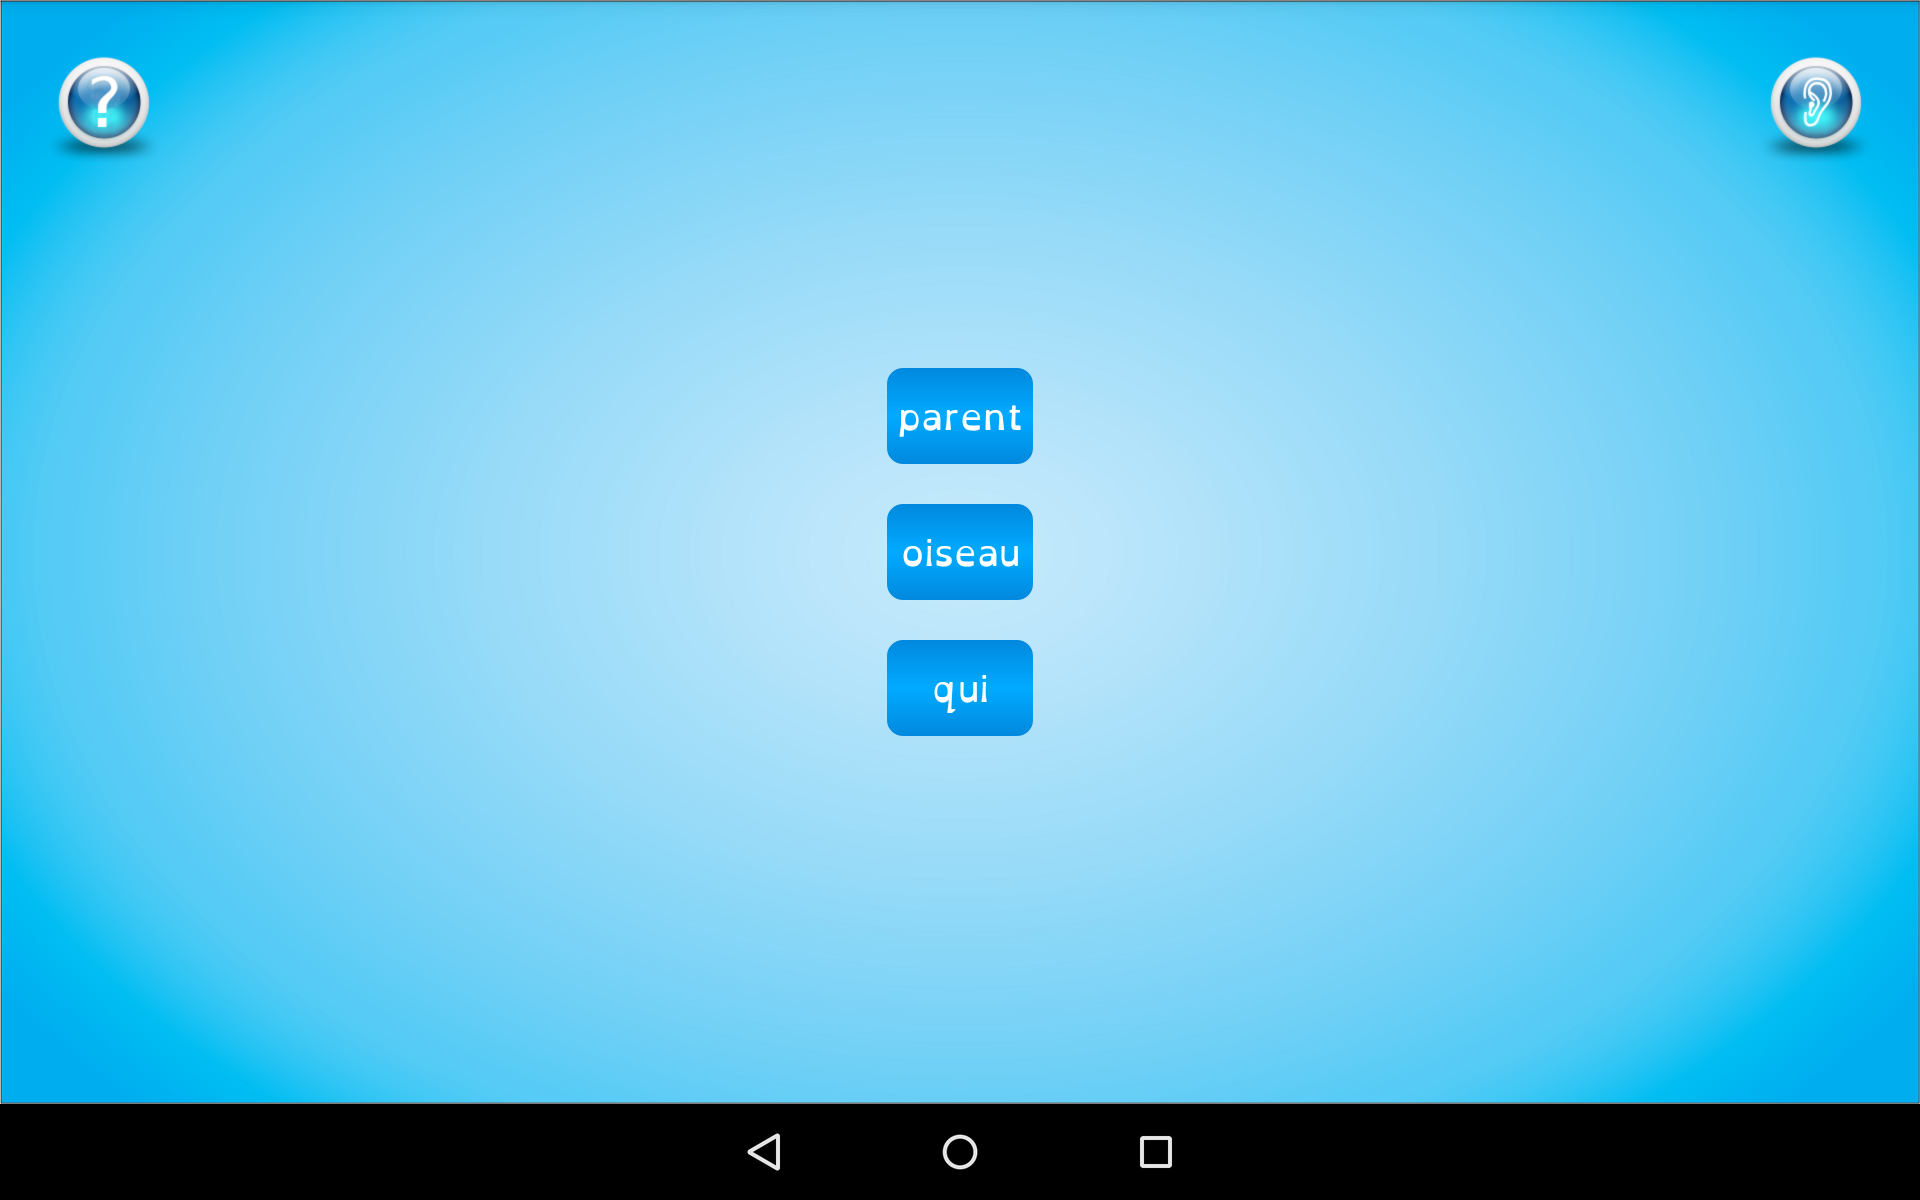
\includegraphics[width=8.5cm]{img/son-start.png}
\caption{Layout principal de l'exercice avec le choix des mots}
\label{son1}
\end{subfigure}
~
\begin{subfigure}[t]{8.5cm}
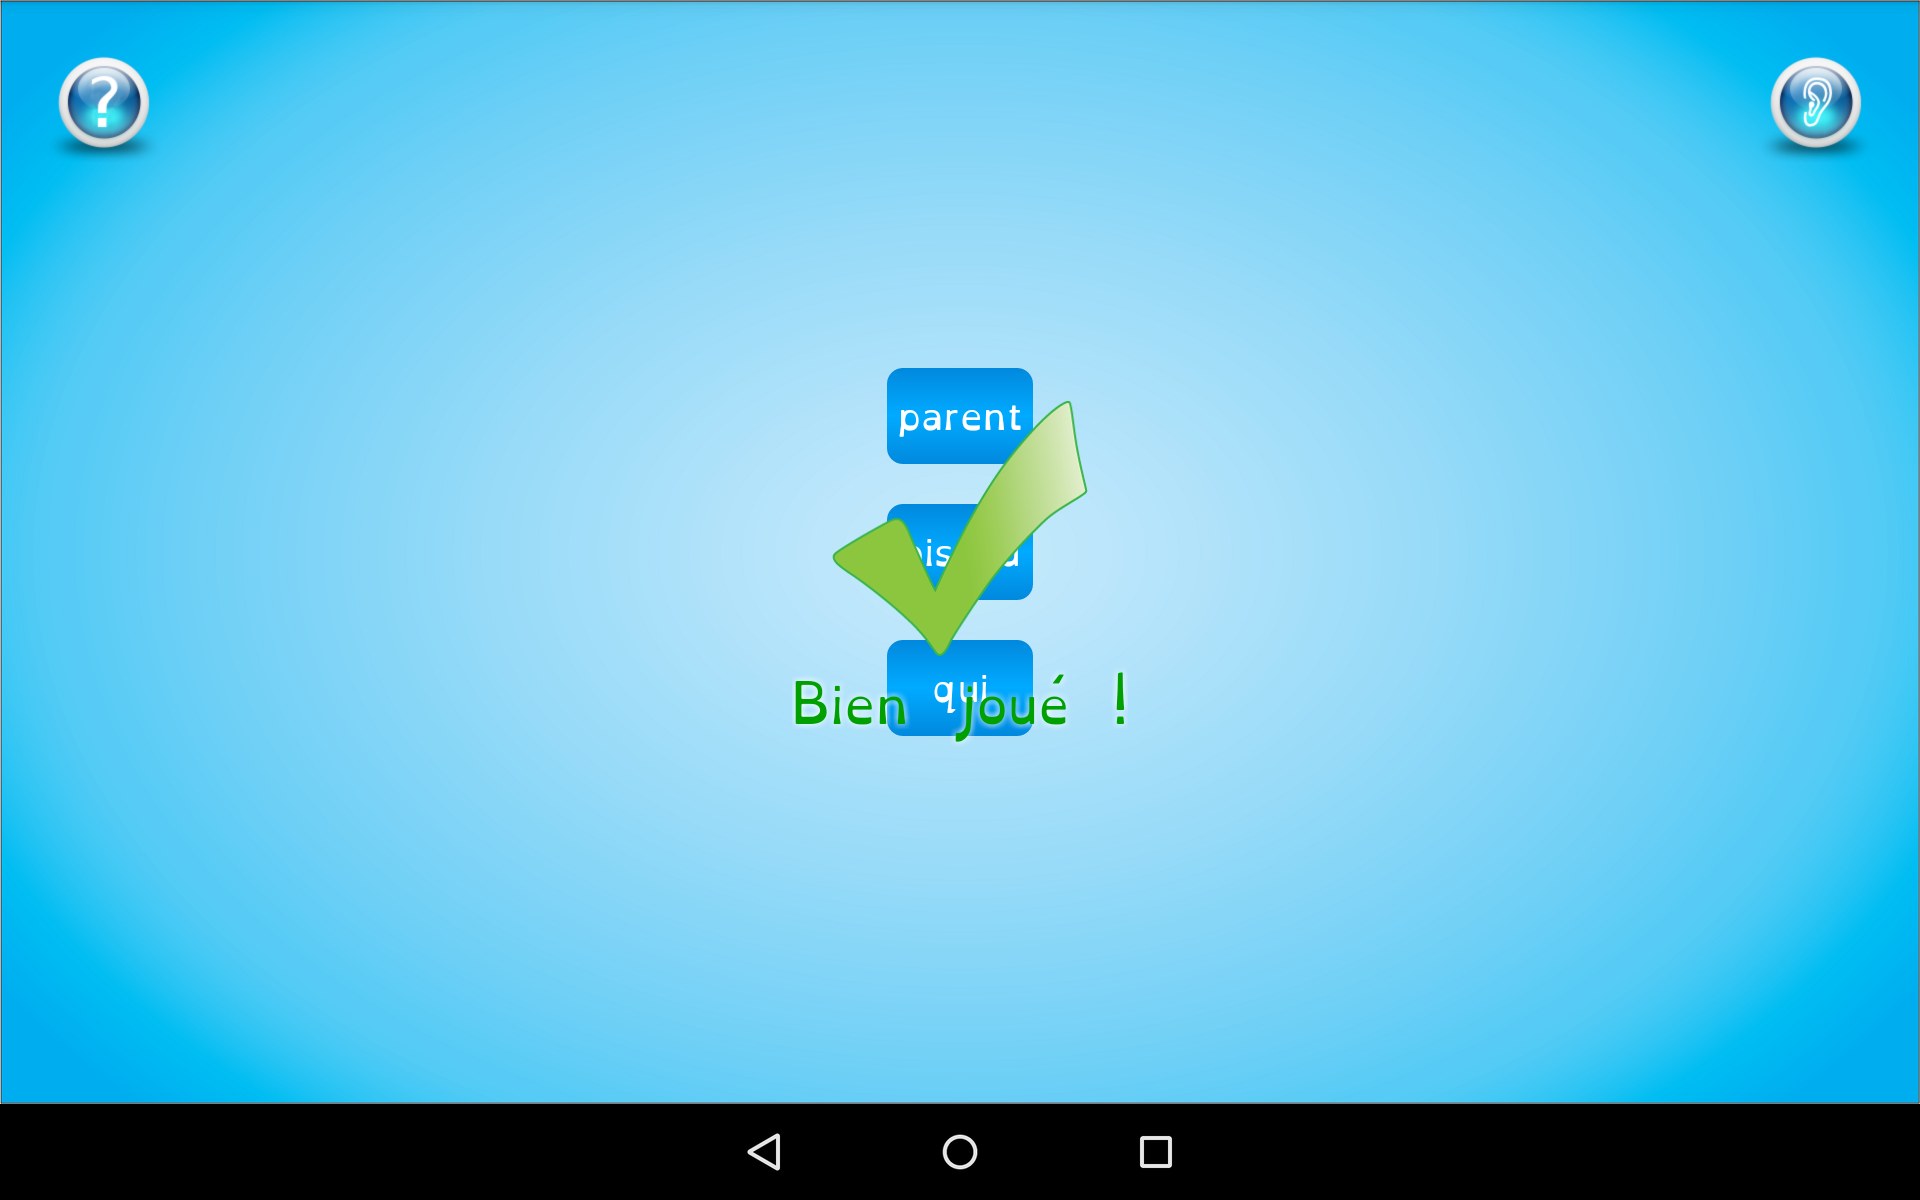
\includegraphics[width=8.5cm]{img/son-ok.png}
\caption{Le mot correct a été sélectionné}
\label{son2}
\end{subfigure}
\caption{Déroulement de l'exercice \textit{Écouter le son}}
\end{figure}

\textit{Écouter le son} n'a pas été l'exercice le plus facile à implémenter, mais ce n'était pas le plus difficile non plus. Ce qui m'a pris le plus de temps était la création des dictionnaires phonétiques. En effet, je dois parcourir manuellement le VOB mot par mot et prononcer ceux-ci afin d'analyser les sons qui les composent et ainsi de définir les codes à ajouter au dictionnaire. La mise en place du code, une fois la logique définie, s'est déroulée sans trop d'encombres.

%A COMPLETER